\chapter{EKLER}\thispagestyle{empty}\setlength{\parindent}{10mm}\setlength{\leftskip}{0mm}\setlength{\parskip}{0pt}

\hypertarget{yapux131-bilgi-formlarux131-ve-ruxf6luxf6ve-uxe7izimleri}{%
\section{Yapı Bilgi Formları ve Rölöve
Çizimleri}\label{yapux131-bilgi-formlarux131-ve-ruxf6luxf6ve-uxe7izimleri}}

\begin{figure}
\centering
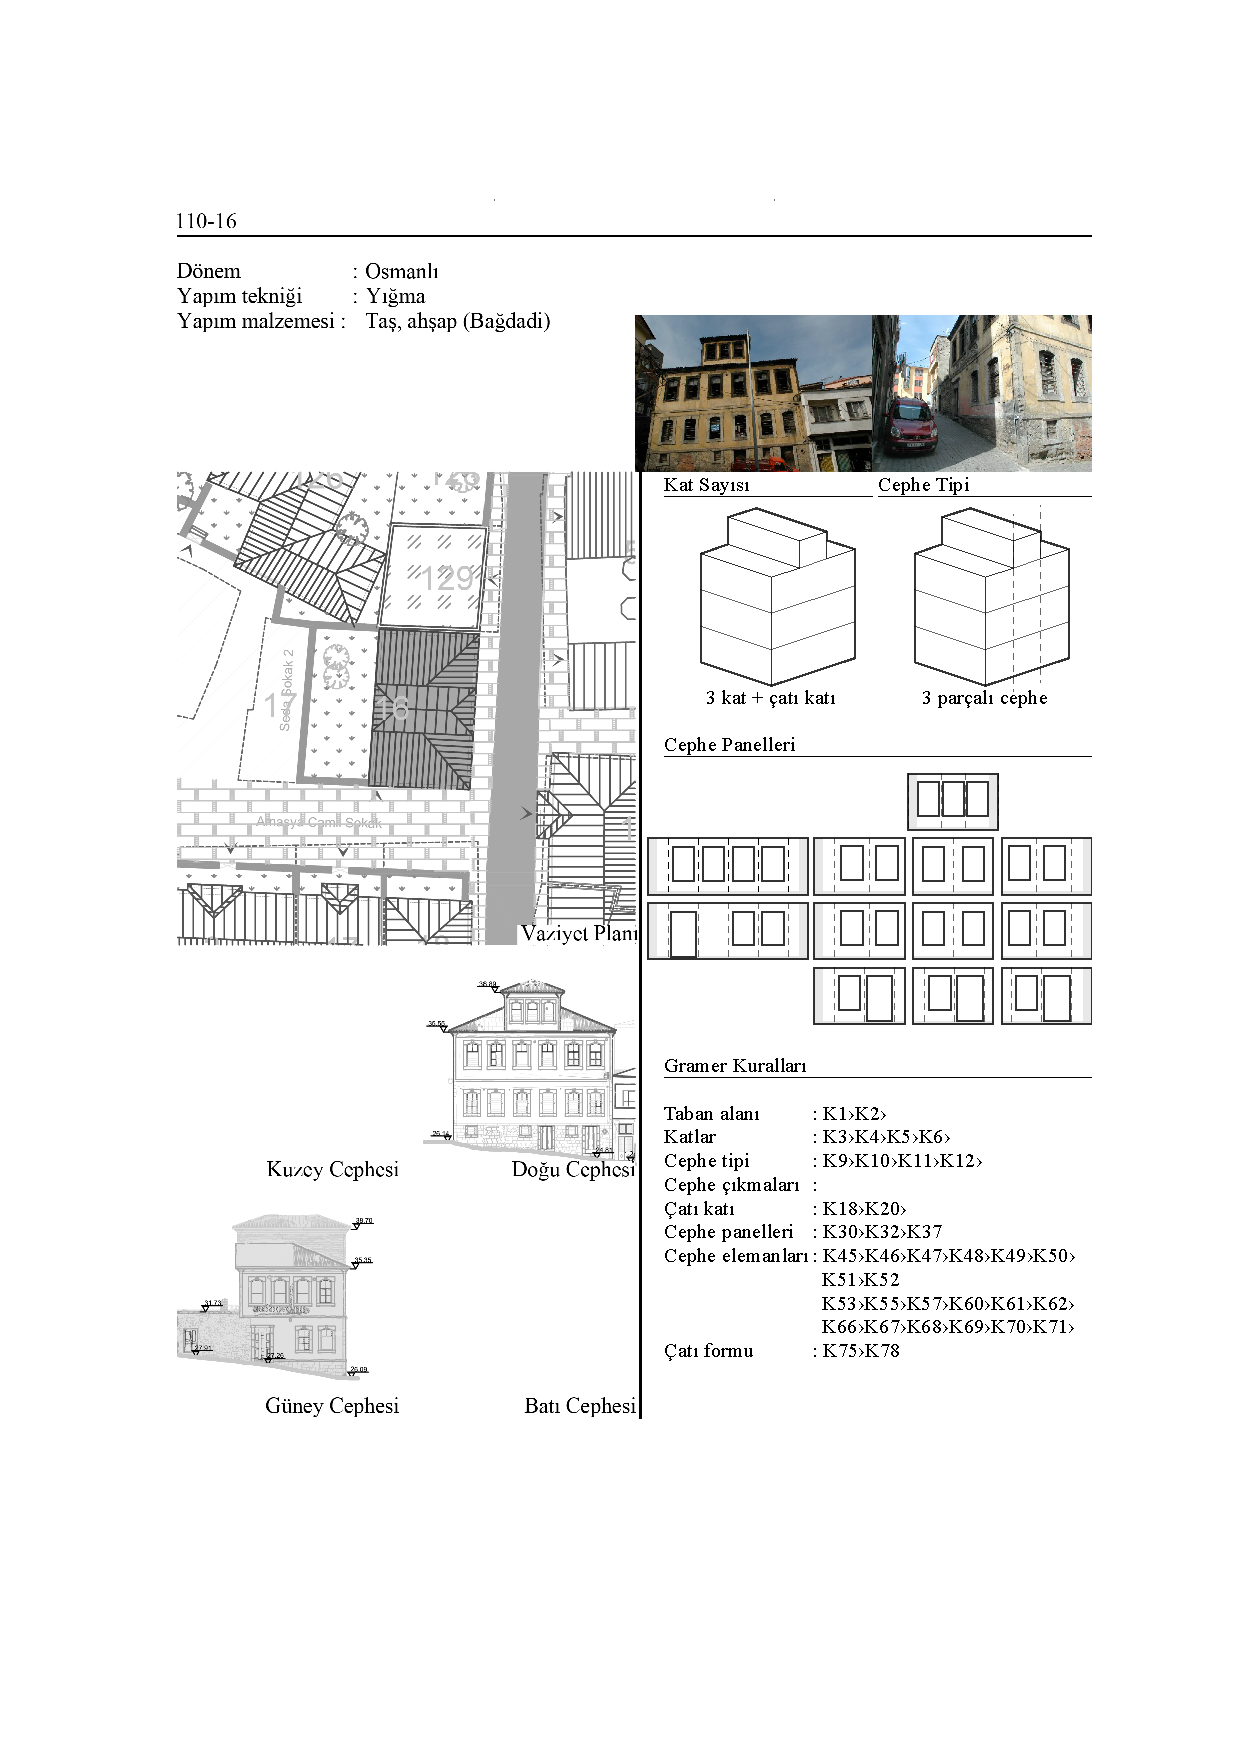
\includegraphics[width=1\textwidth,height=\textheight]{source/figures/BilgiFormlari/110-16.pdf}
\caption{110 ada 16 parsele ait yapı bilgi formu.}
\end{figure}

\begin{figure}
\centering
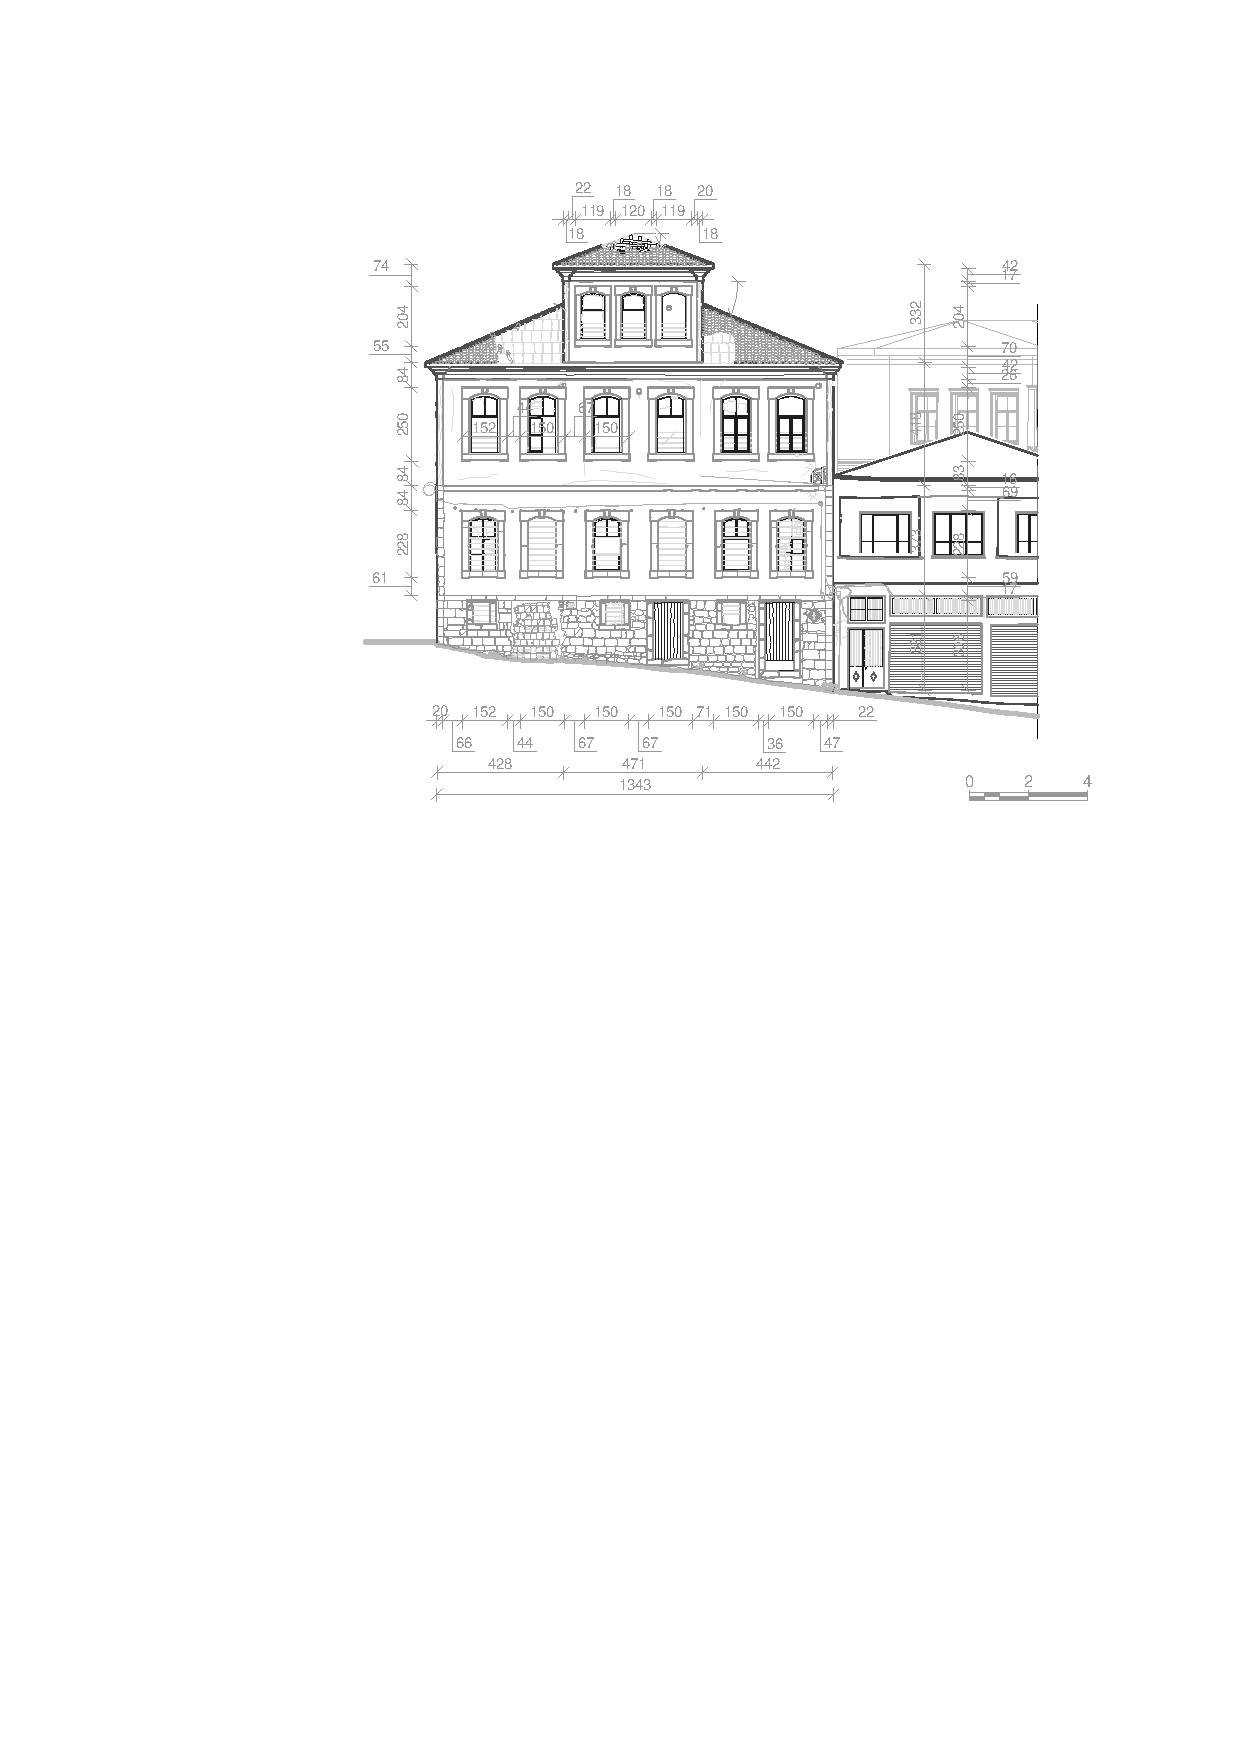
\includegraphics[width=1\textwidth,height=\textheight]{source/figures/Roloveler/R110-16.pdf}
\caption{110 ada 16 parsele ait rölöve çizimi.}
\end{figure}

\begin{figure}
\centering
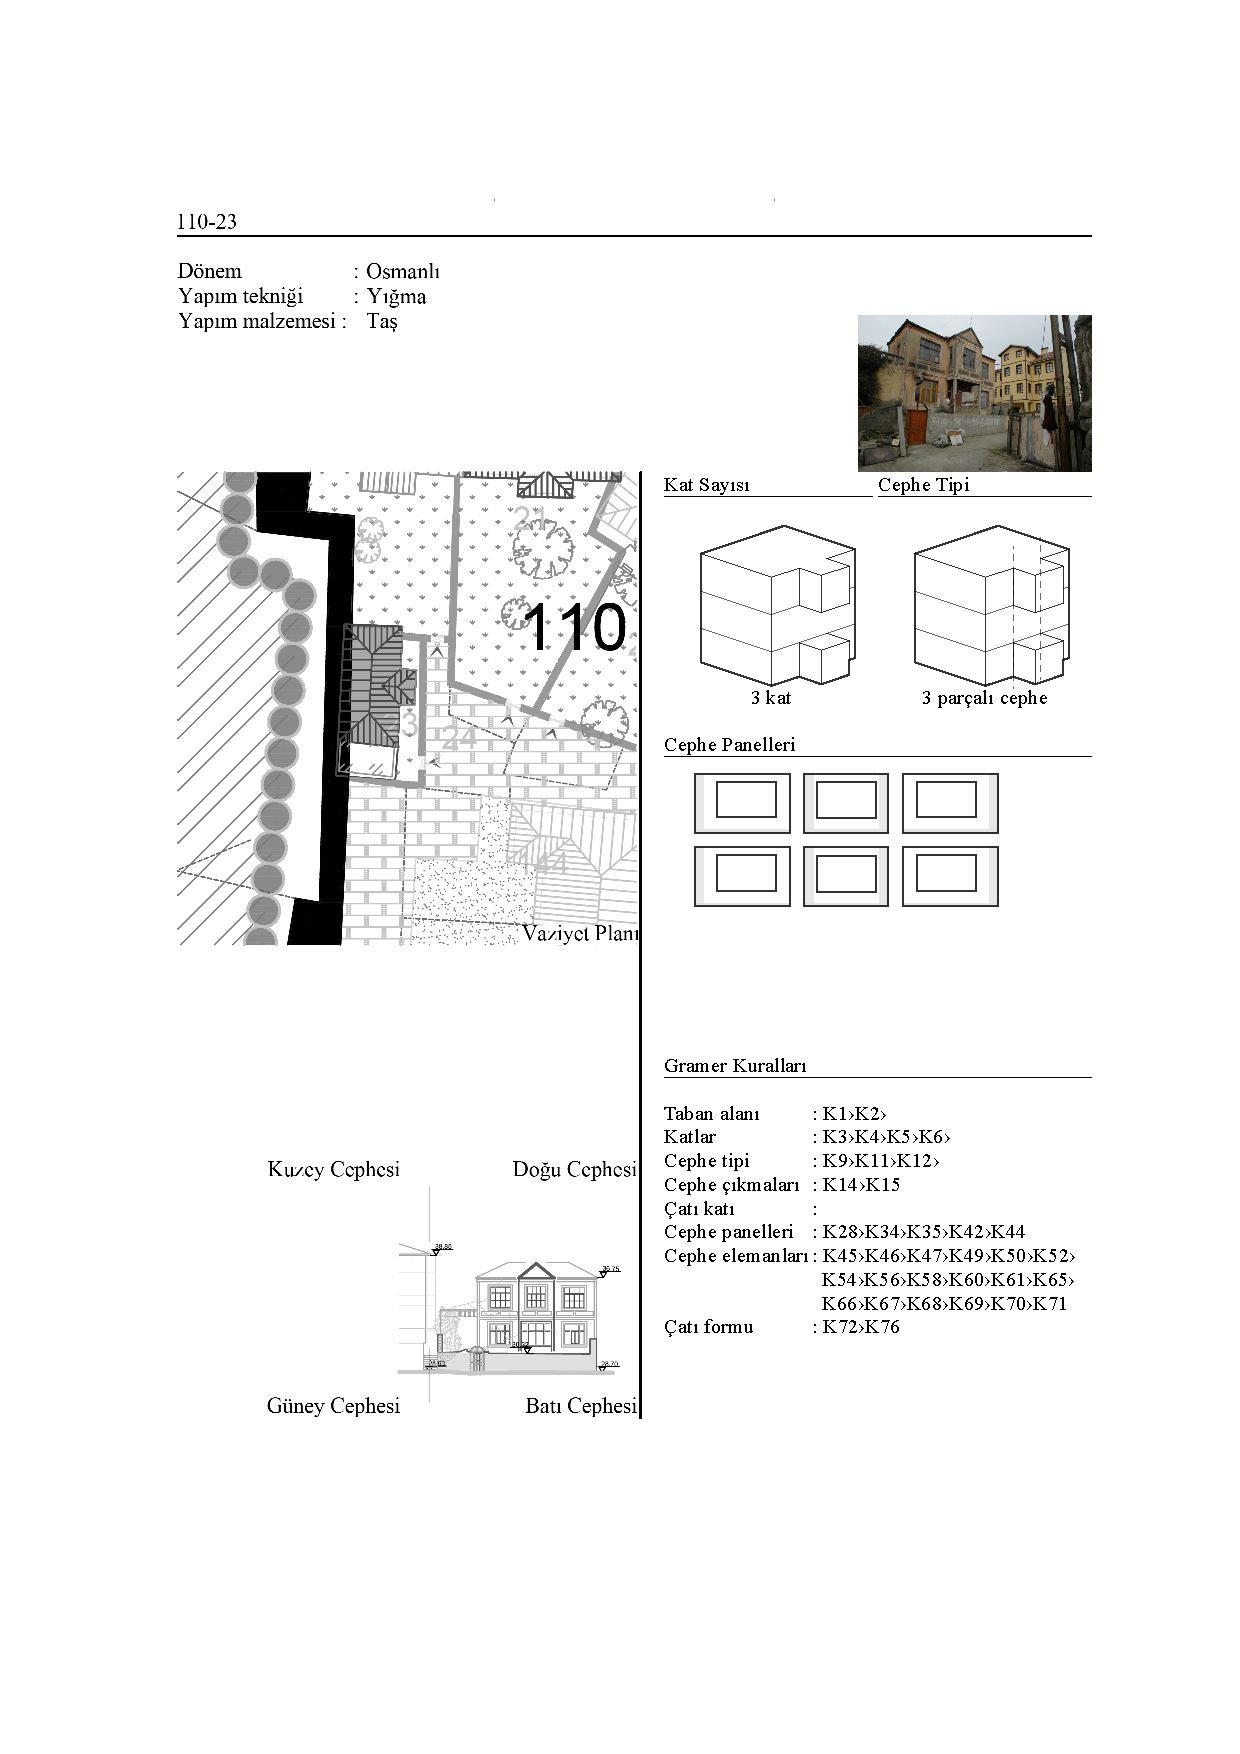
\includegraphics[width=1\textwidth,height=\textheight]{source/figures/BilgiFormlari/110-23.pdf}
\caption{110 ada 23 parsele ait yapı bilgi formu.}
\end{figure}

\begin{figure}
\centering
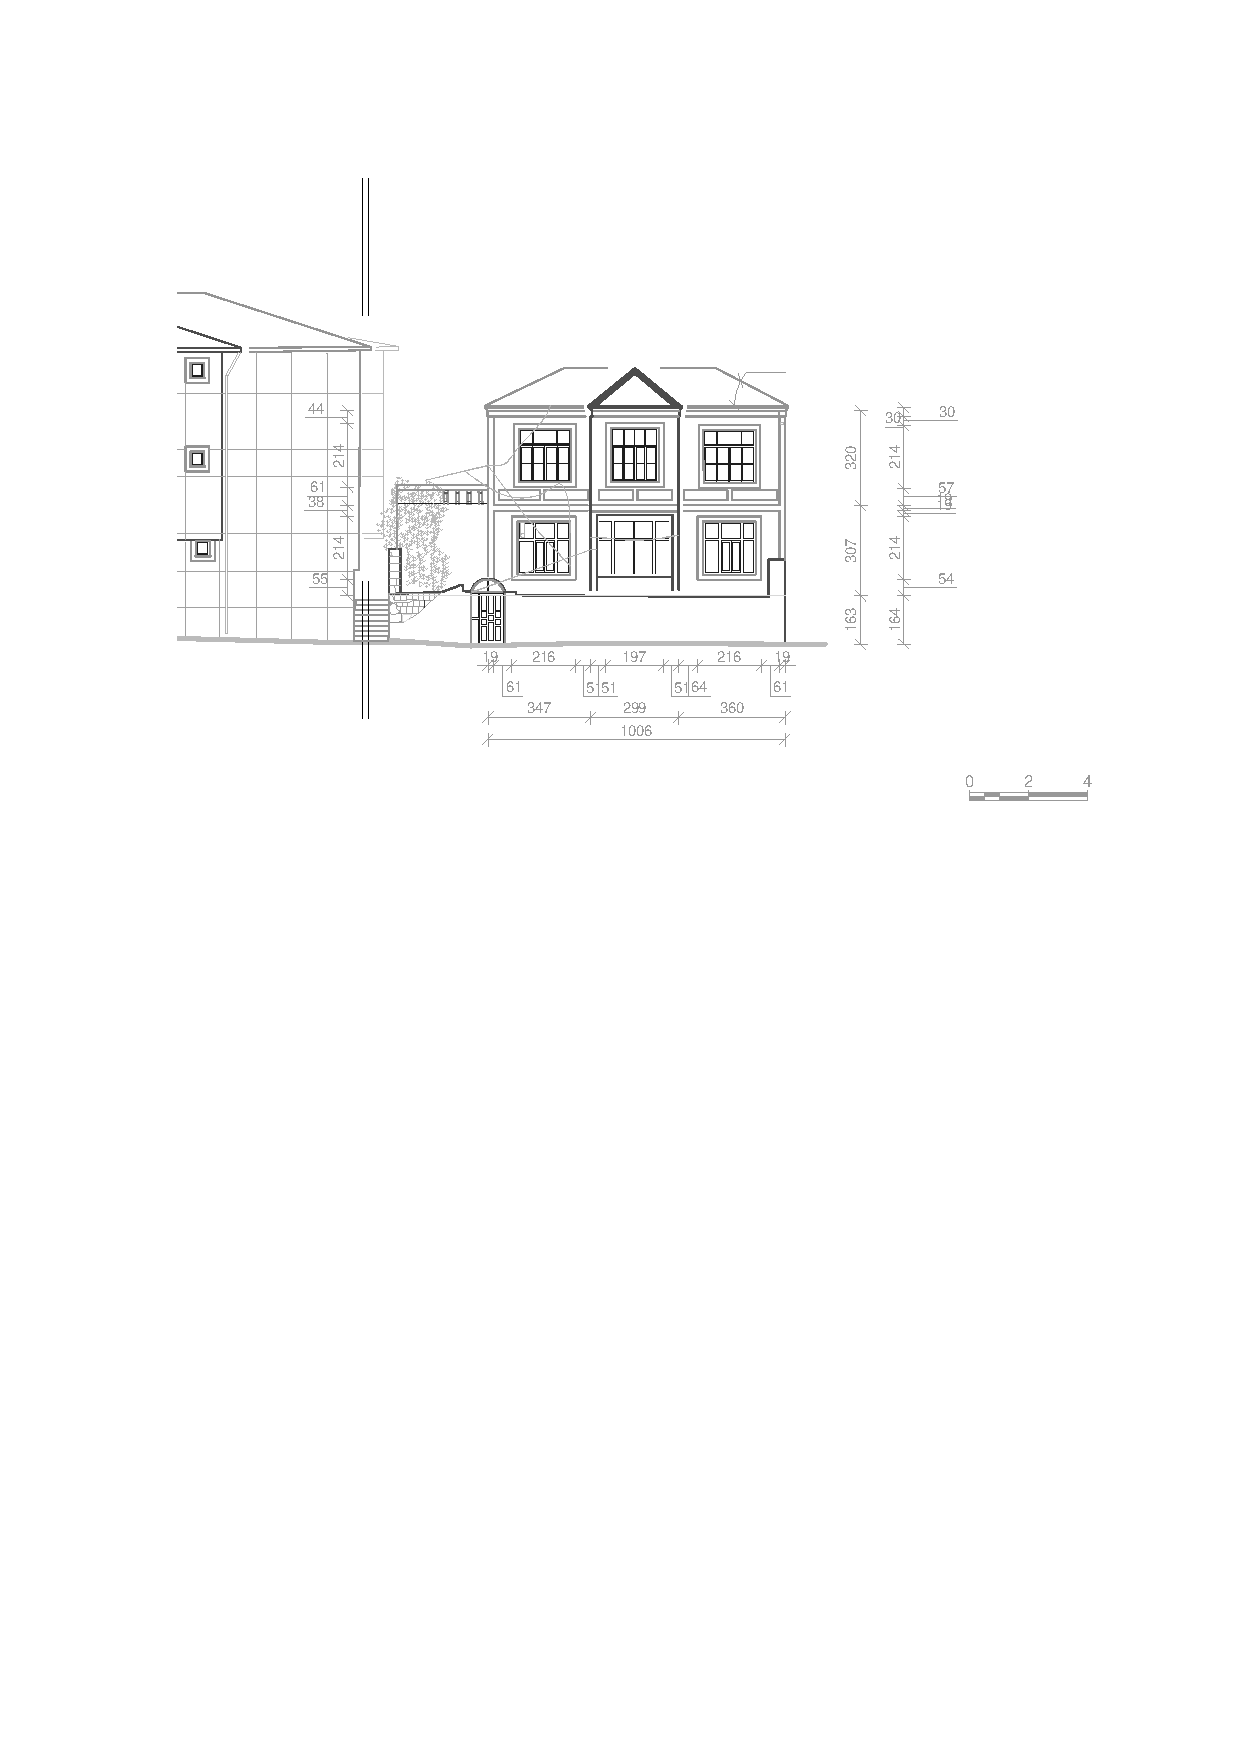
\includegraphics[width=1\textwidth,height=\textheight]{source/figures/Roloveler/R110-23.pdf}
\caption{110 ada 23 parsele ait rölöve çizimi.}
\end{figure}

\begin{figure}
\centering
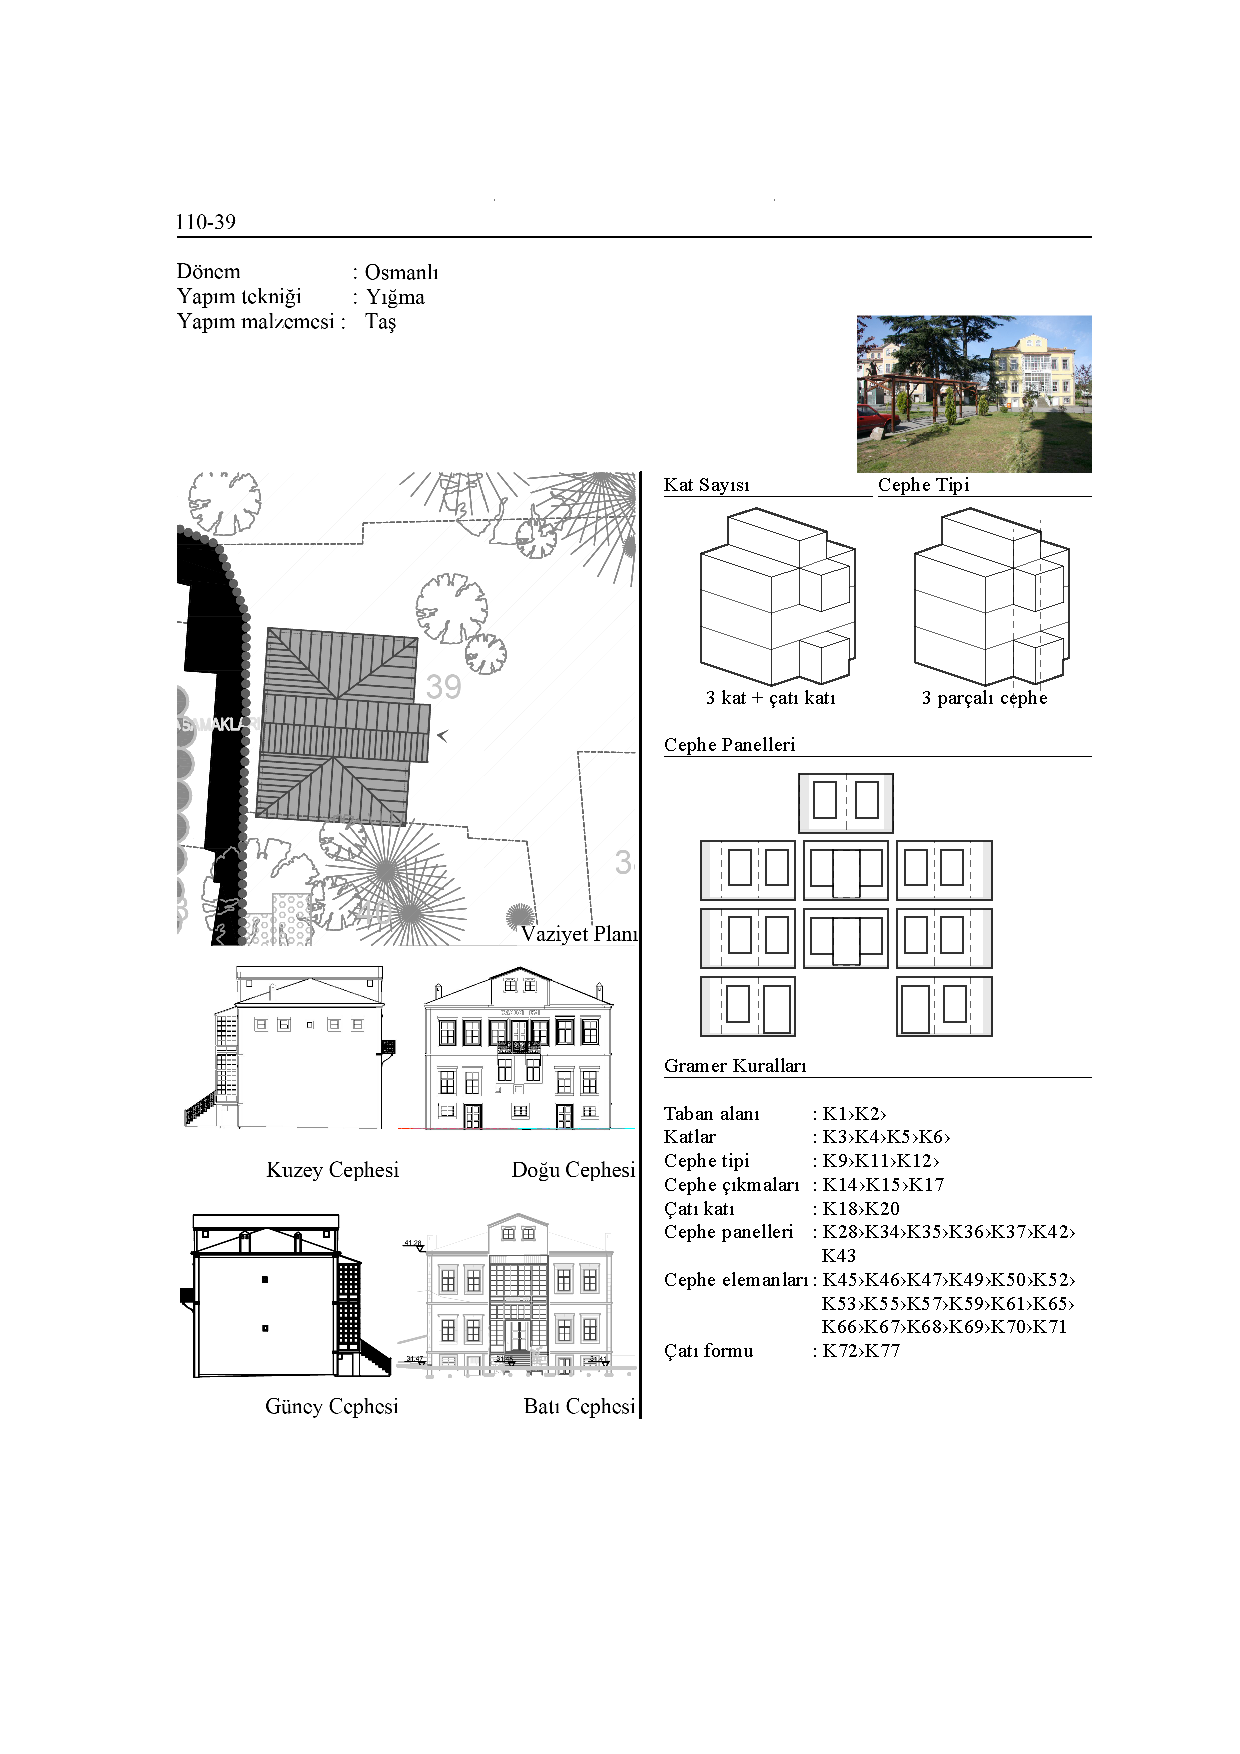
\includegraphics[width=1\textwidth,height=\textheight]{source/figures/BilgiFormlari/110-39.pdf}
\caption{110 ada 39 parsele ait yapı bilgi formu.}
\end{figure}

\begin{figure}
\centering
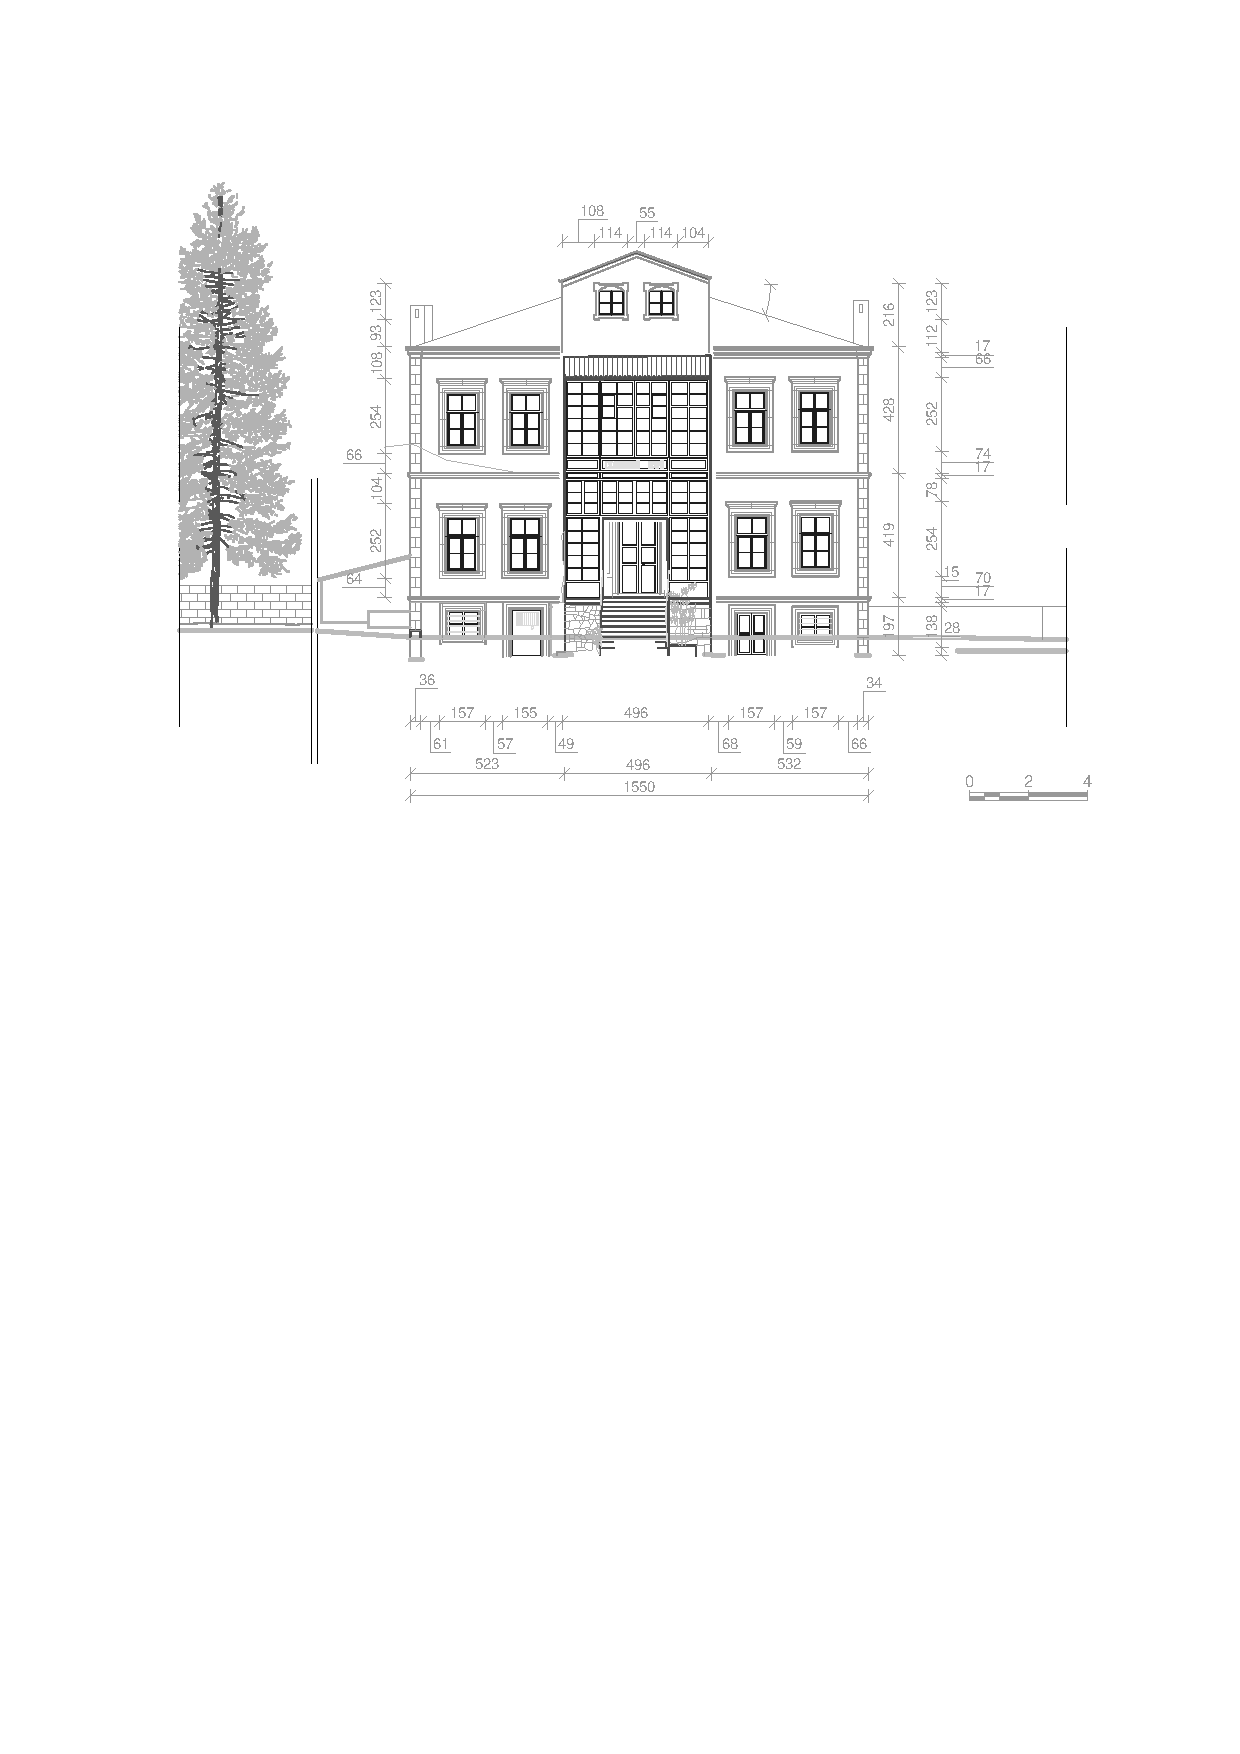
\includegraphics[width=1\textwidth,height=\textheight]{source/figures/Roloveler/R110-39.pdf}
\caption{110 ada 39 parsele ait rölöve çizimi.}
\end{figure}

\begin{figure}
\centering
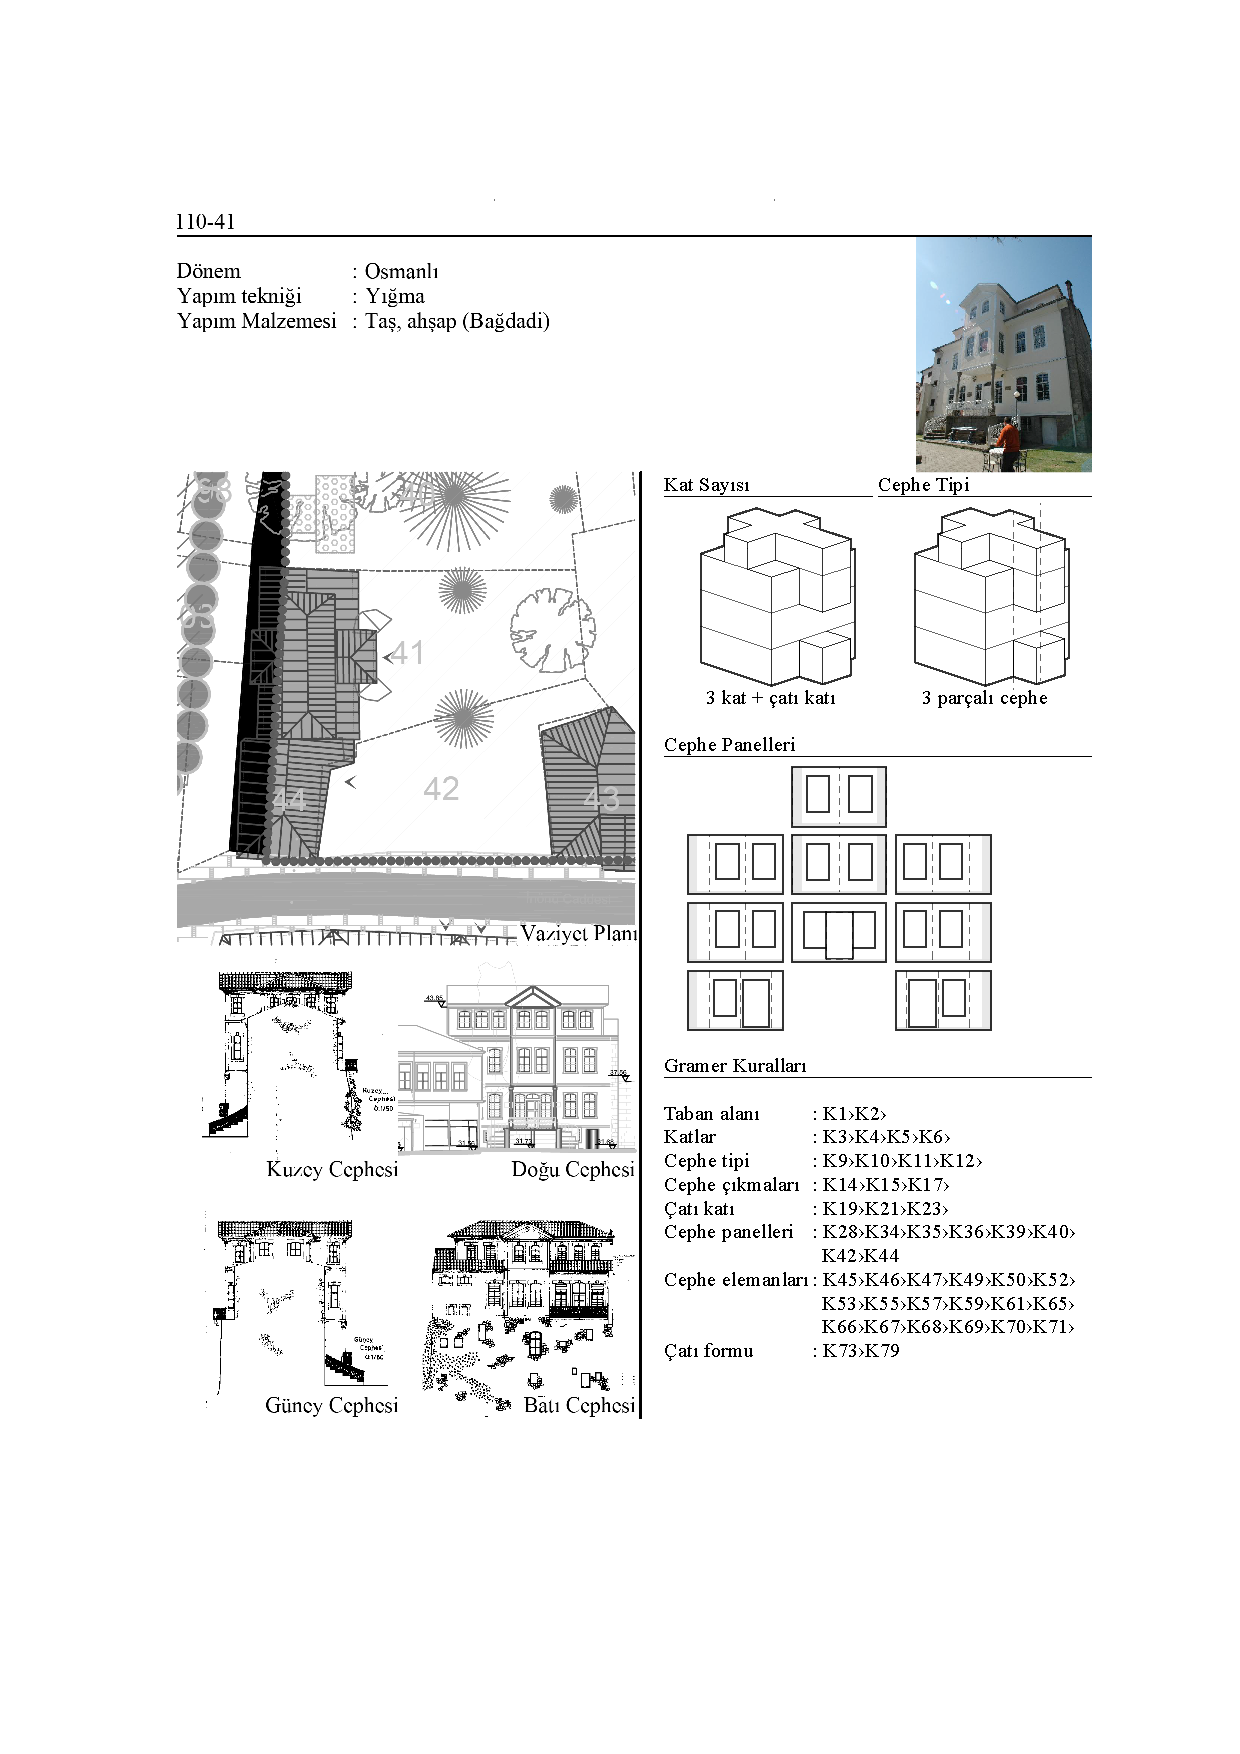
\includegraphics[width=1\textwidth,height=\textheight]{source/figures/BilgiFormlari/110-41.pdf}
\caption{110 ada 41 parsele ait yapı bilgi formu.}
\end{figure}

\begin{figure}
\centering
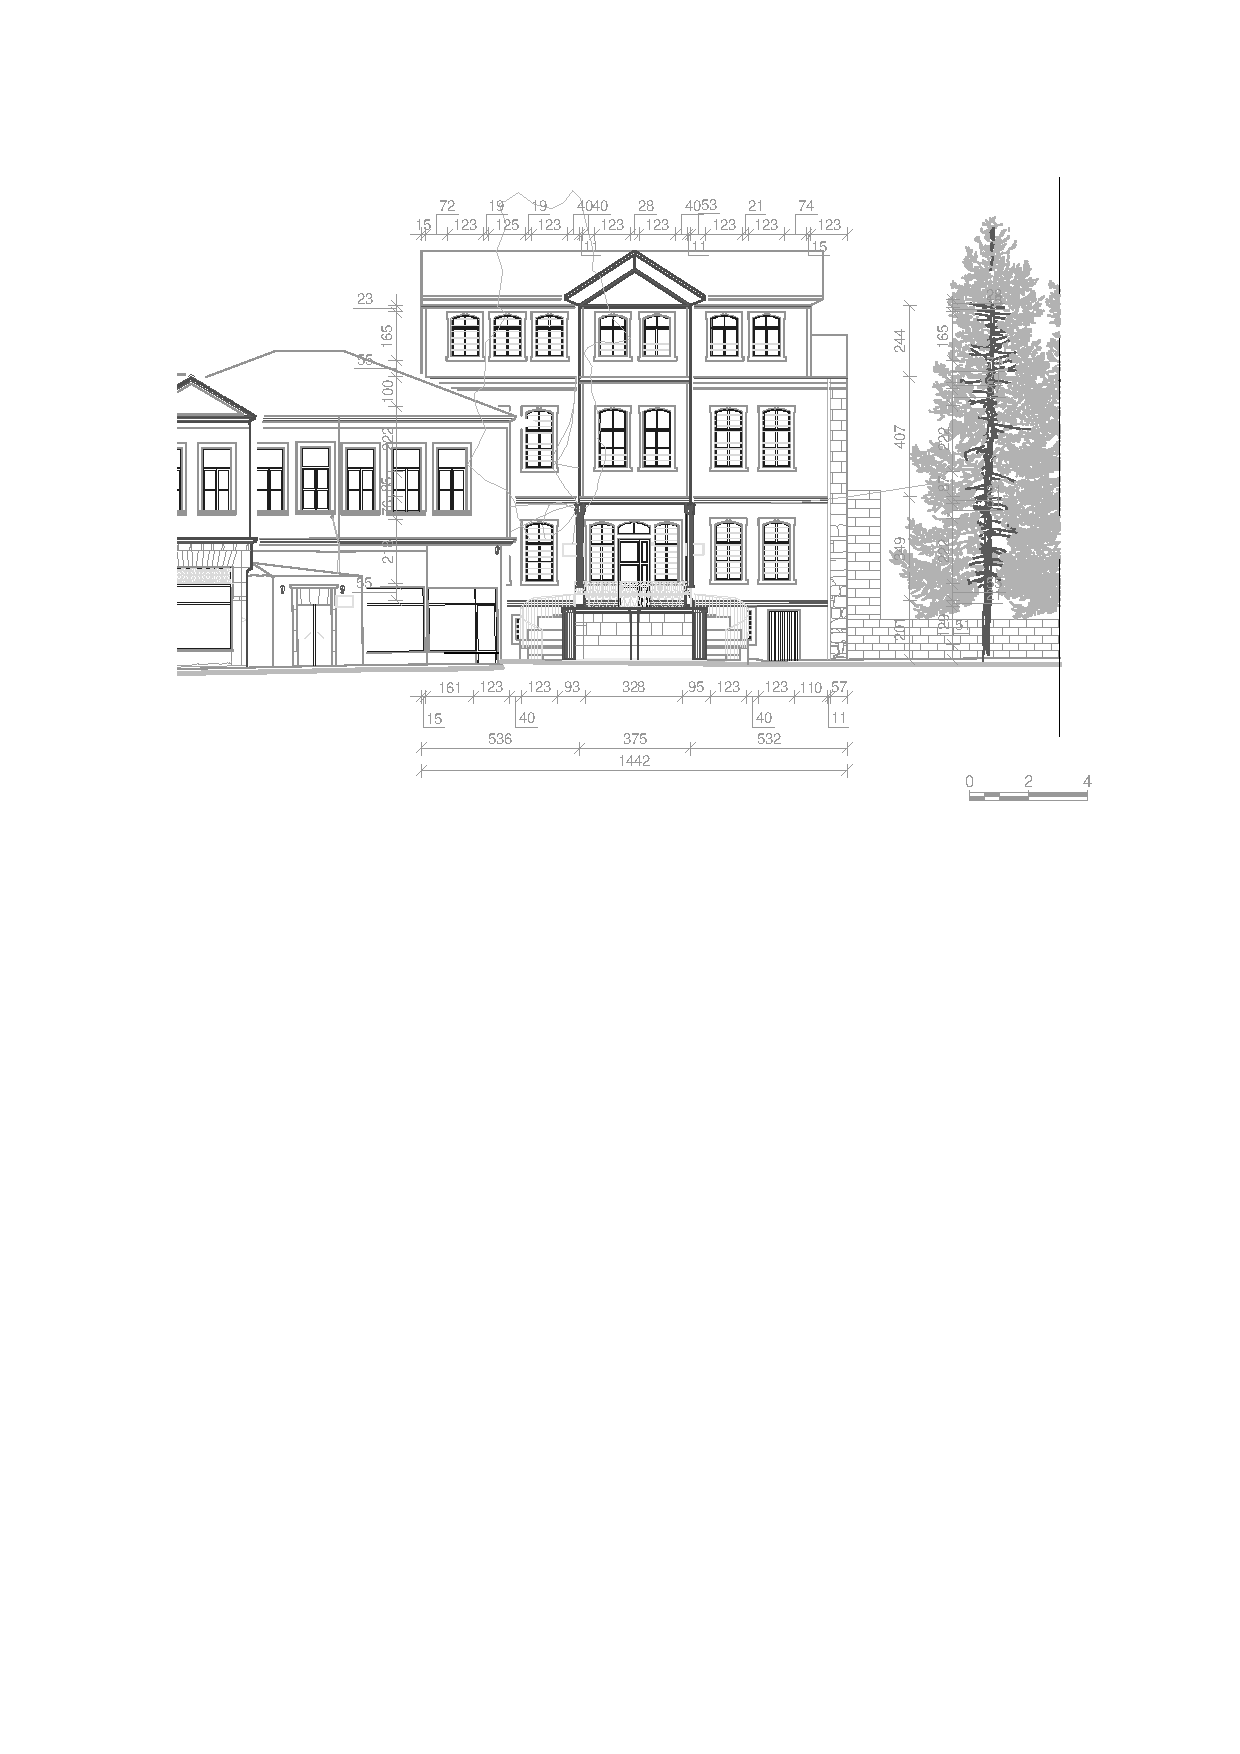
\includegraphics[width=1\textwidth,height=\textheight]{source/figures/Roloveler/R110-41.pdf}
\caption{110 ada 41 parsele ait rölöve çizimi.}
\end{figure}

\begin{figure}
\centering
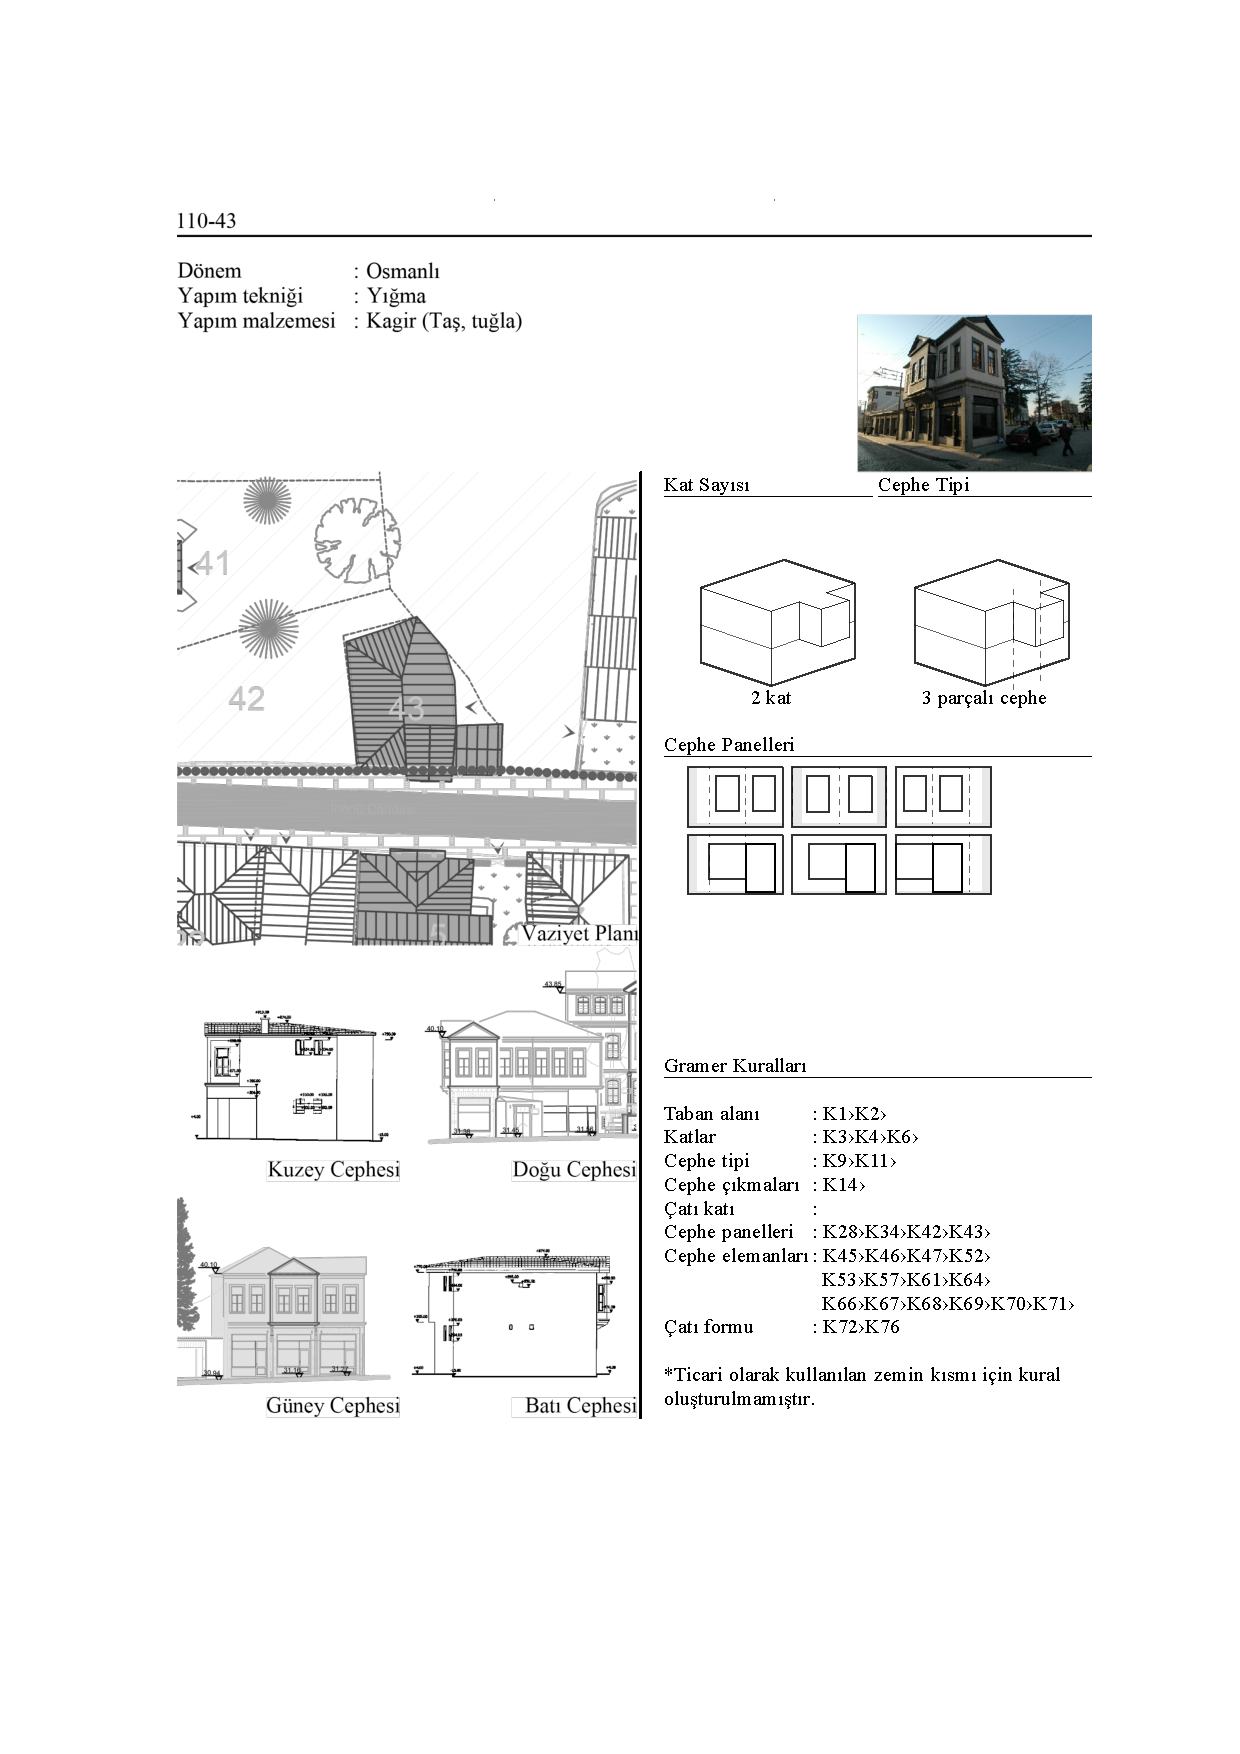
\includegraphics[width=1\textwidth,height=\textheight]{source/figures/BilgiFormlari/110-43.pdf}
\caption{110 ada 43 parsele ait yapı bilgi formu.}
\end{figure}

\begin{figure}
\centering
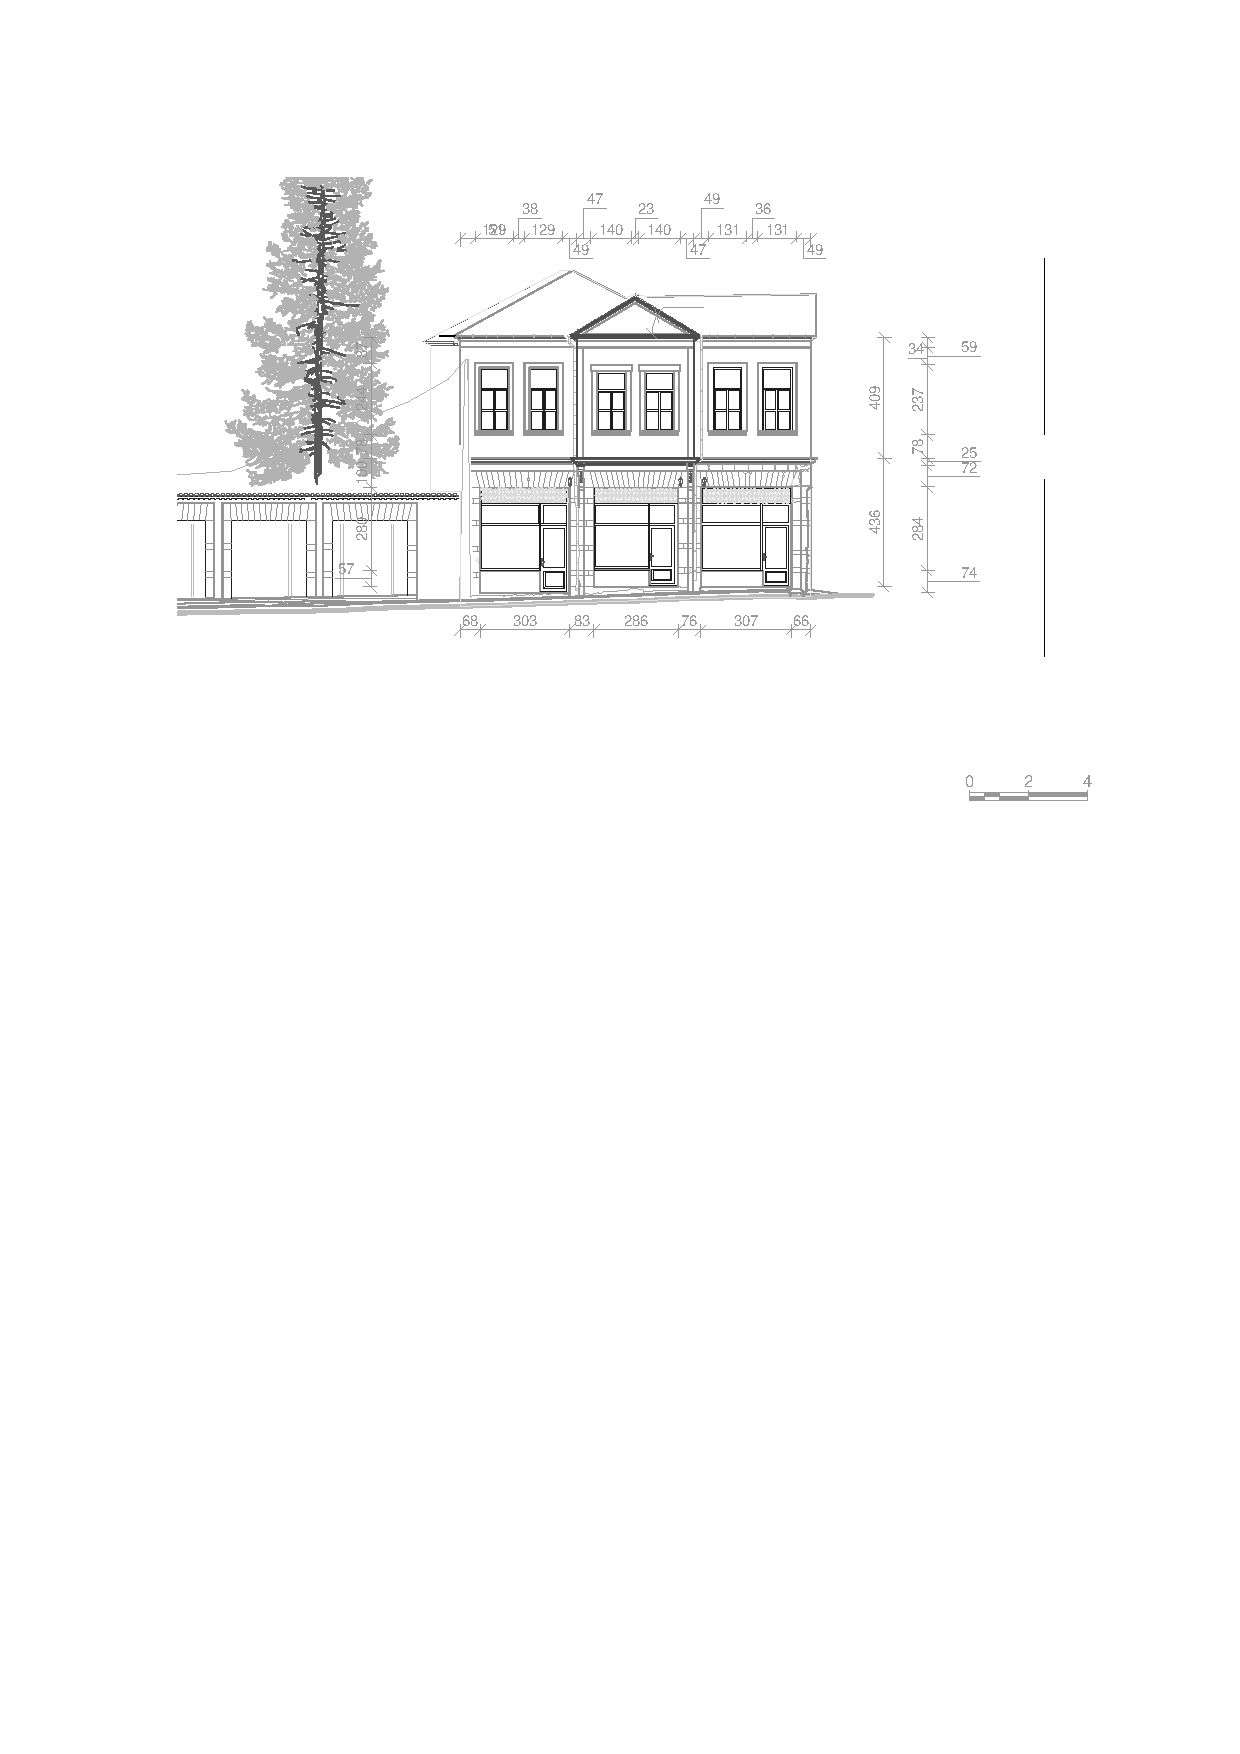
\includegraphics[width=1\textwidth,height=\textheight]{source/figures/Roloveler/R110-43.pdf}
\caption{110 ada 43 parsele ait rölöve çizimi.}
\end{figure}

\begin{figure}
\centering
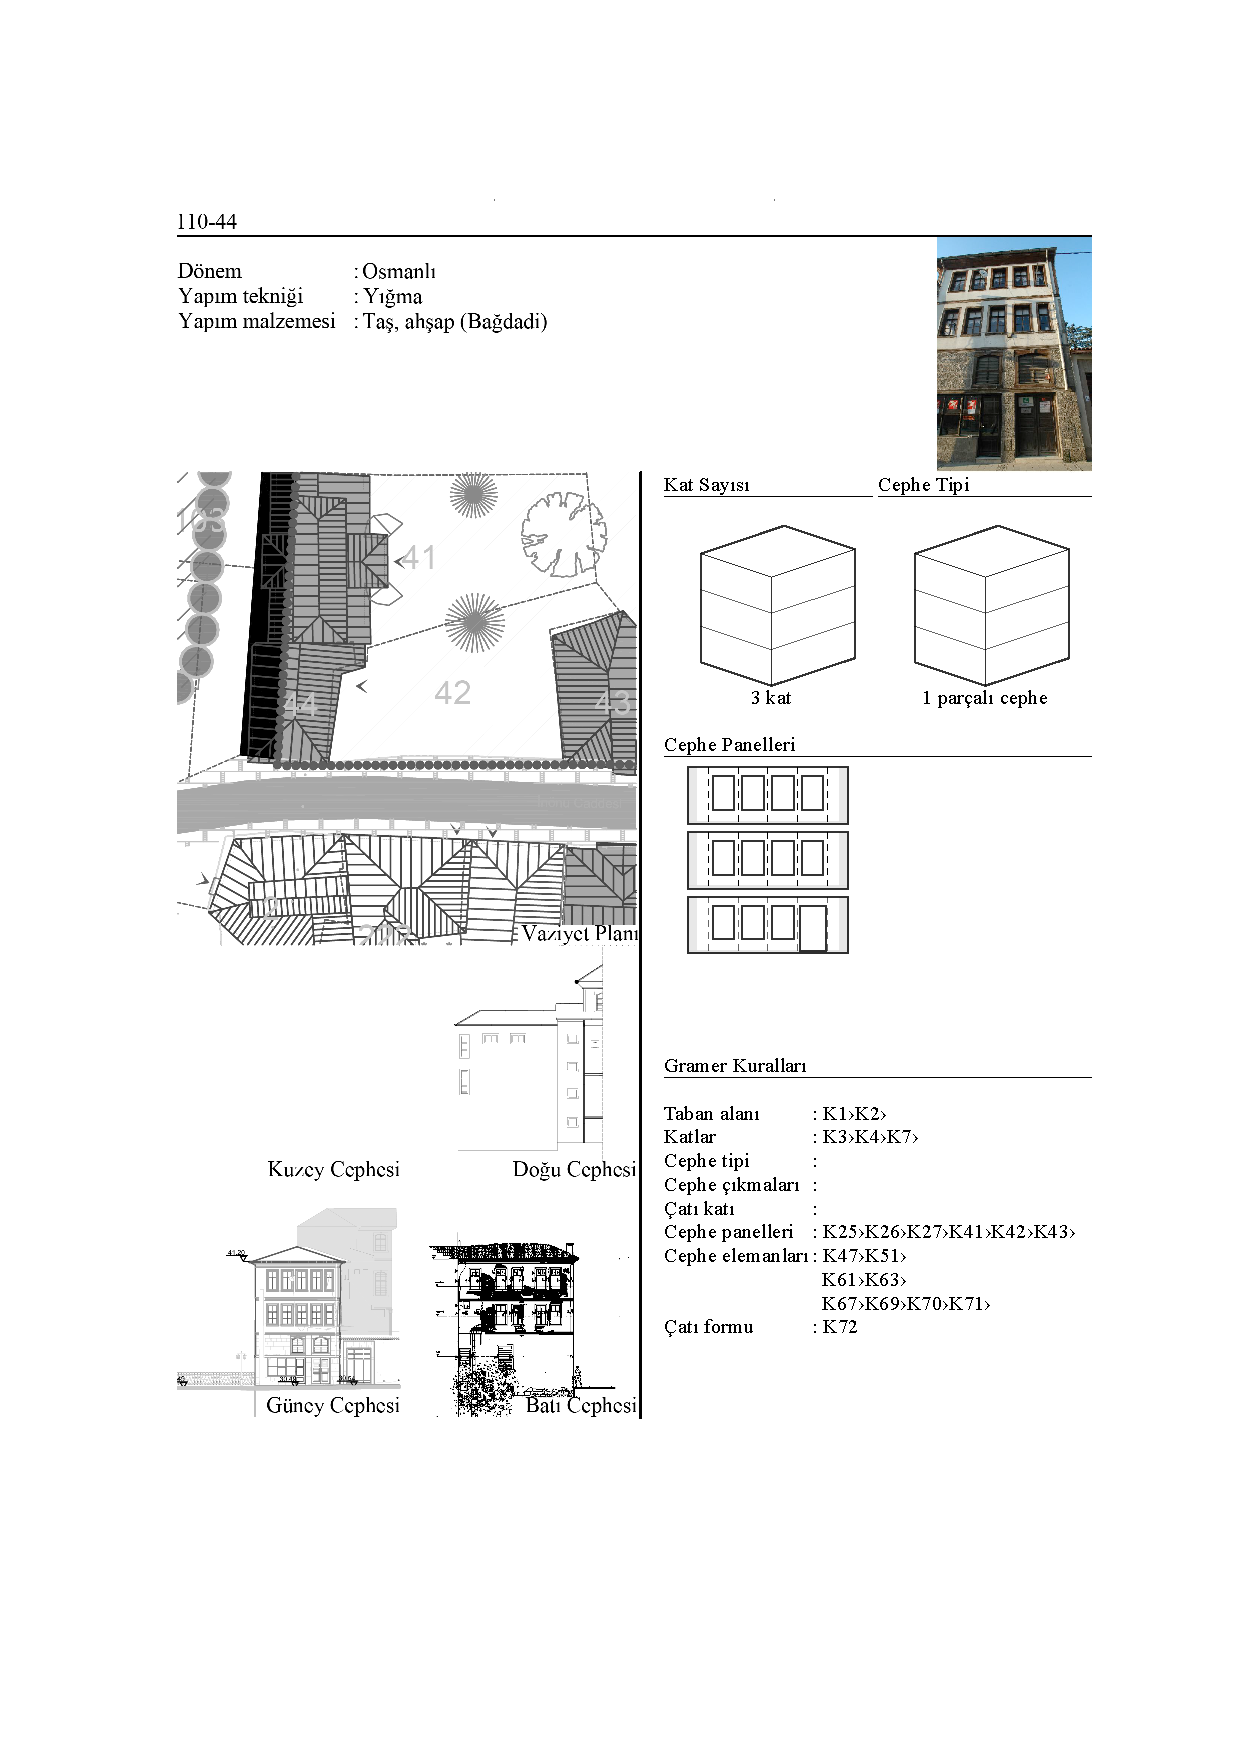
\includegraphics[width=1\textwidth,height=\textheight]{source/figures/BilgiFormlari/110-44.pdf}
\caption{110 ada 44 parsele ait yapı bilgi formu.}
\end{figure}

\begin{figure}
\centering
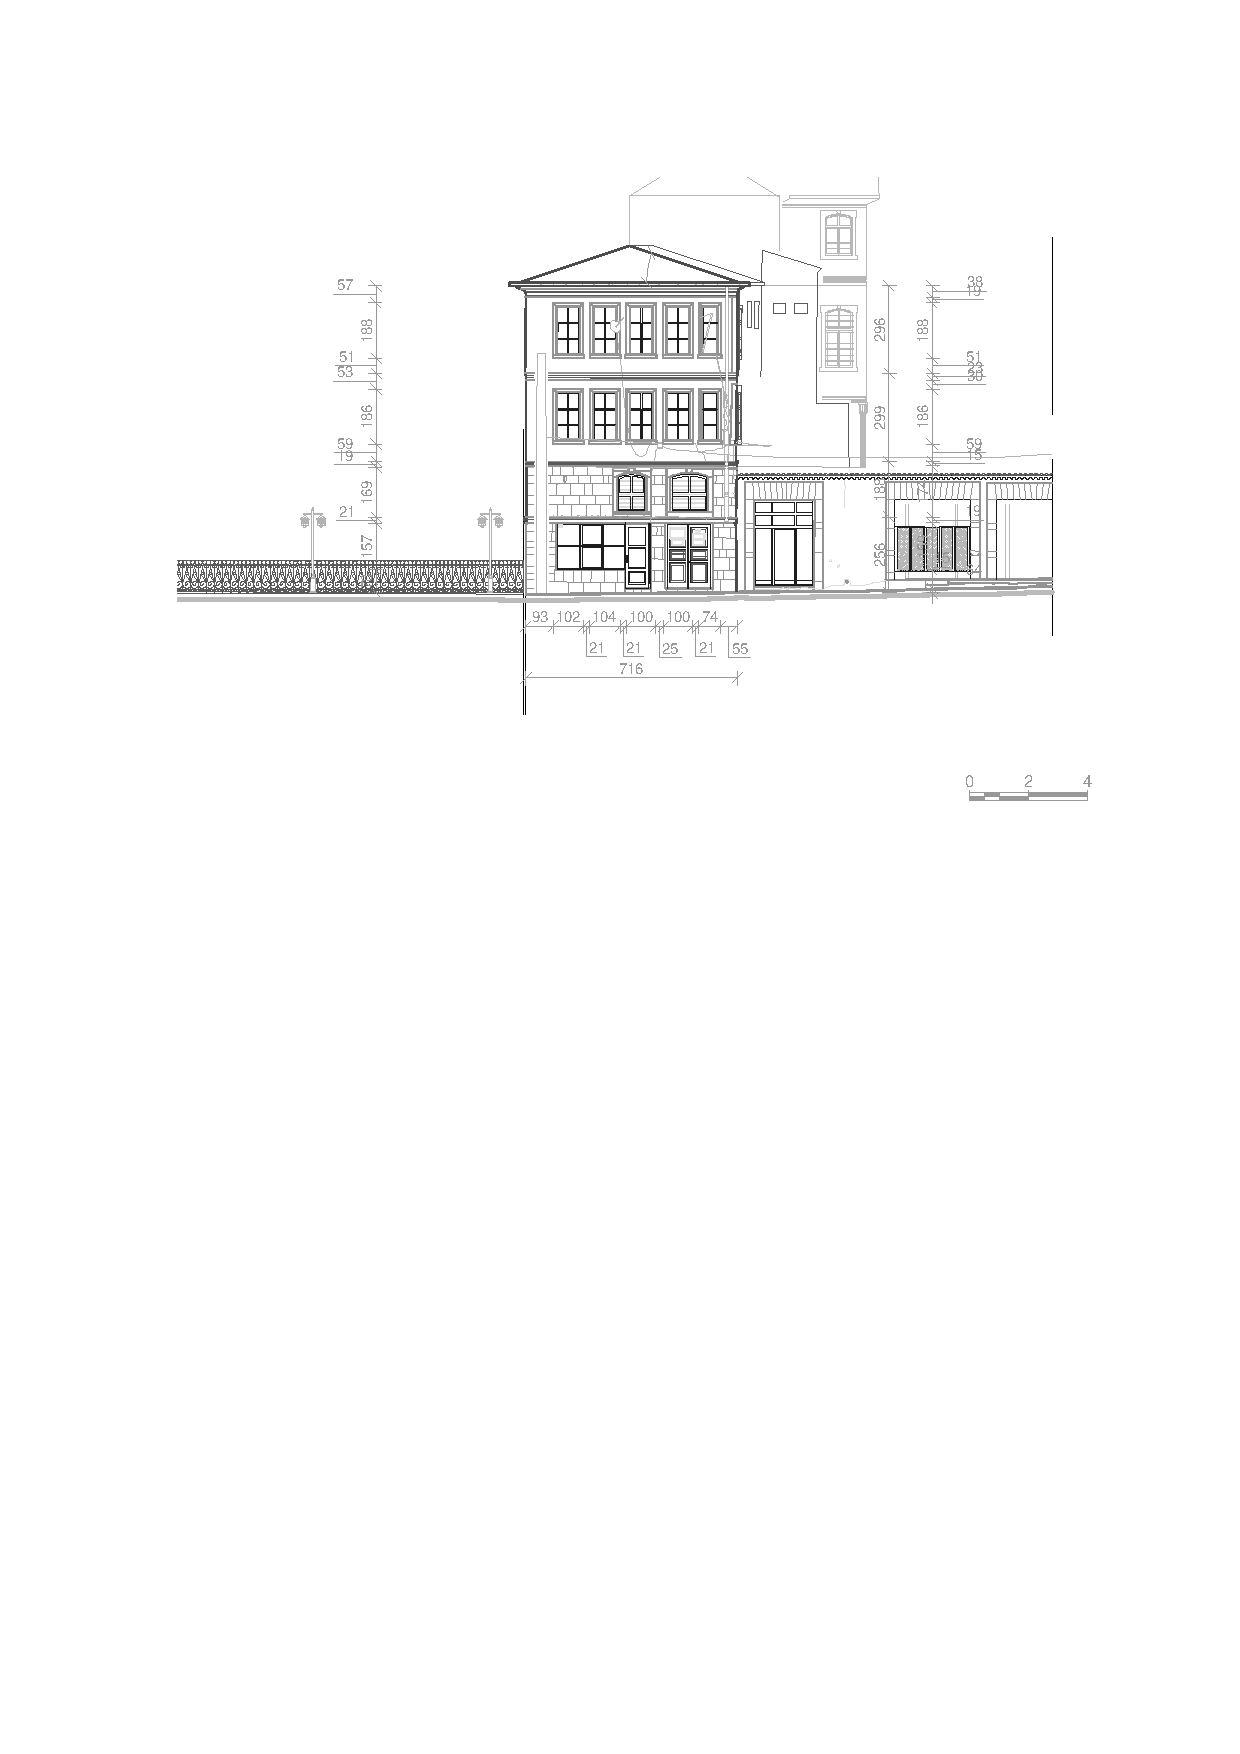
\includegraphics[width=1\textwidth,height=\textheight]{source/figures/Roloveler/R110-44.pdf}
\caption{110 ada 44 parsele ait rölöve çizimi.}
\end{figure}

\begin{figure}
\centering
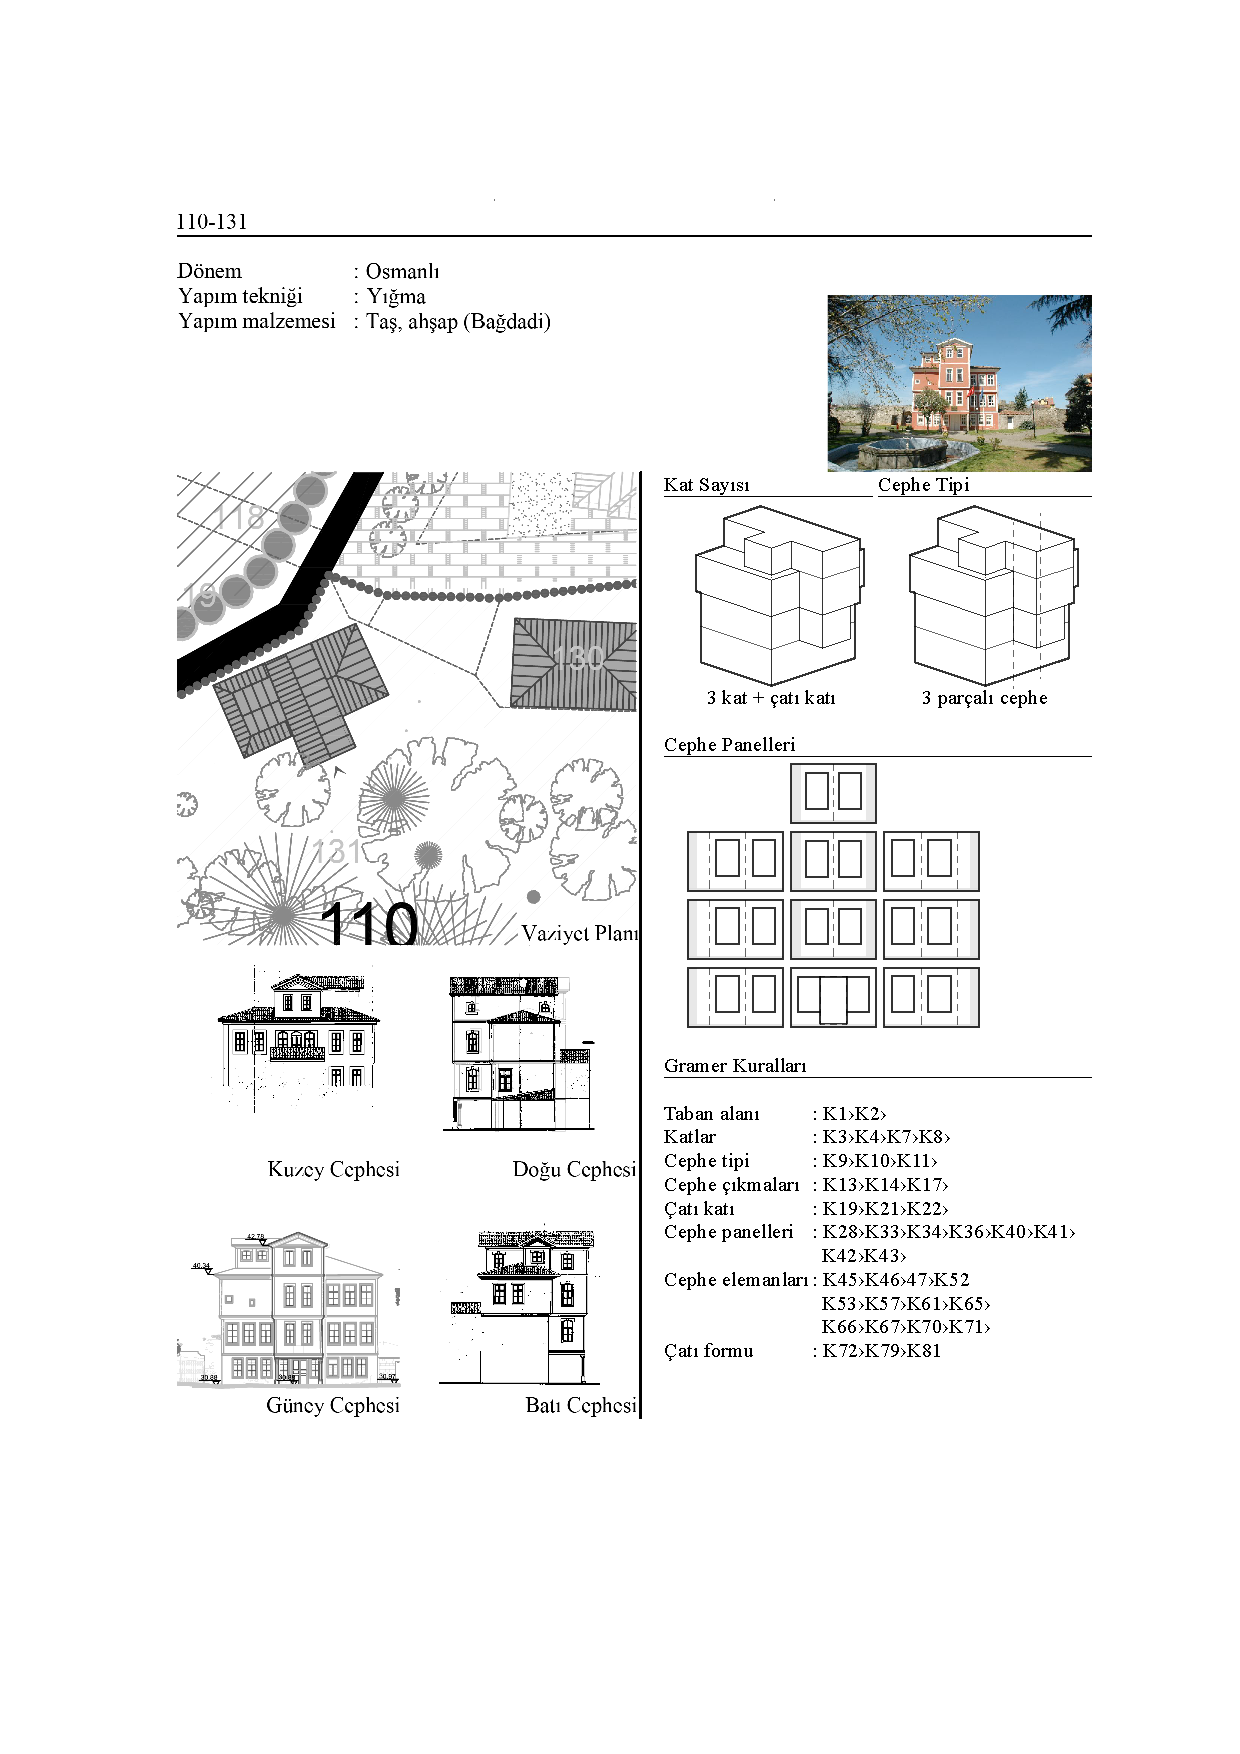
\includegraphics[width=1\textwidth,height=\textheight]{source/figures/BilgiFormlari/110-131.pdf}
\caption{110 ada 131 parsele ait yapı bilgi formu.}
\end{figure}

\begin{figure}
\centering
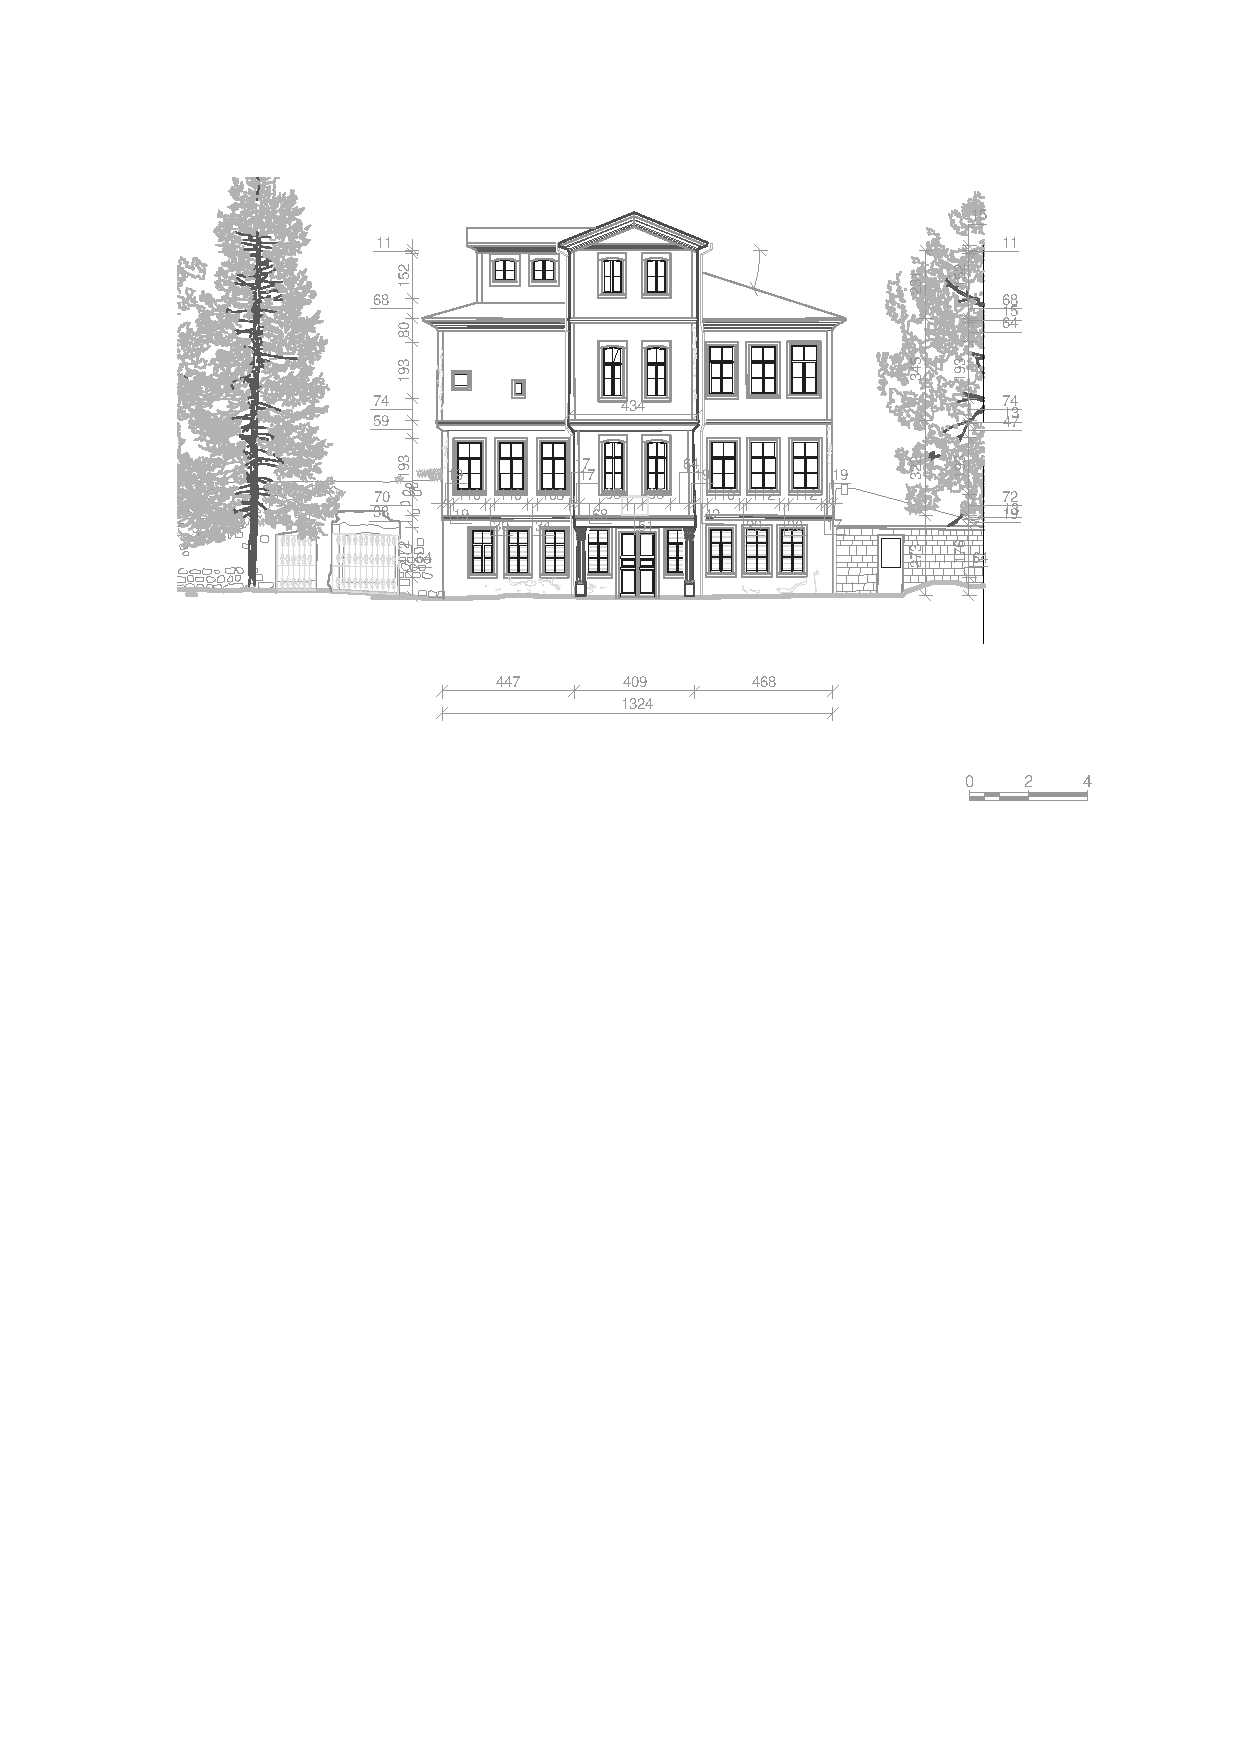
\includegraphics[width=1\textwidth,height=\textheight]{source/figures/Roloveler/R110-131.pdf}
\caption{110 ada 131 parsele ait rölöve çizimi.}
\end{figure}

\begin{figure}
\centering
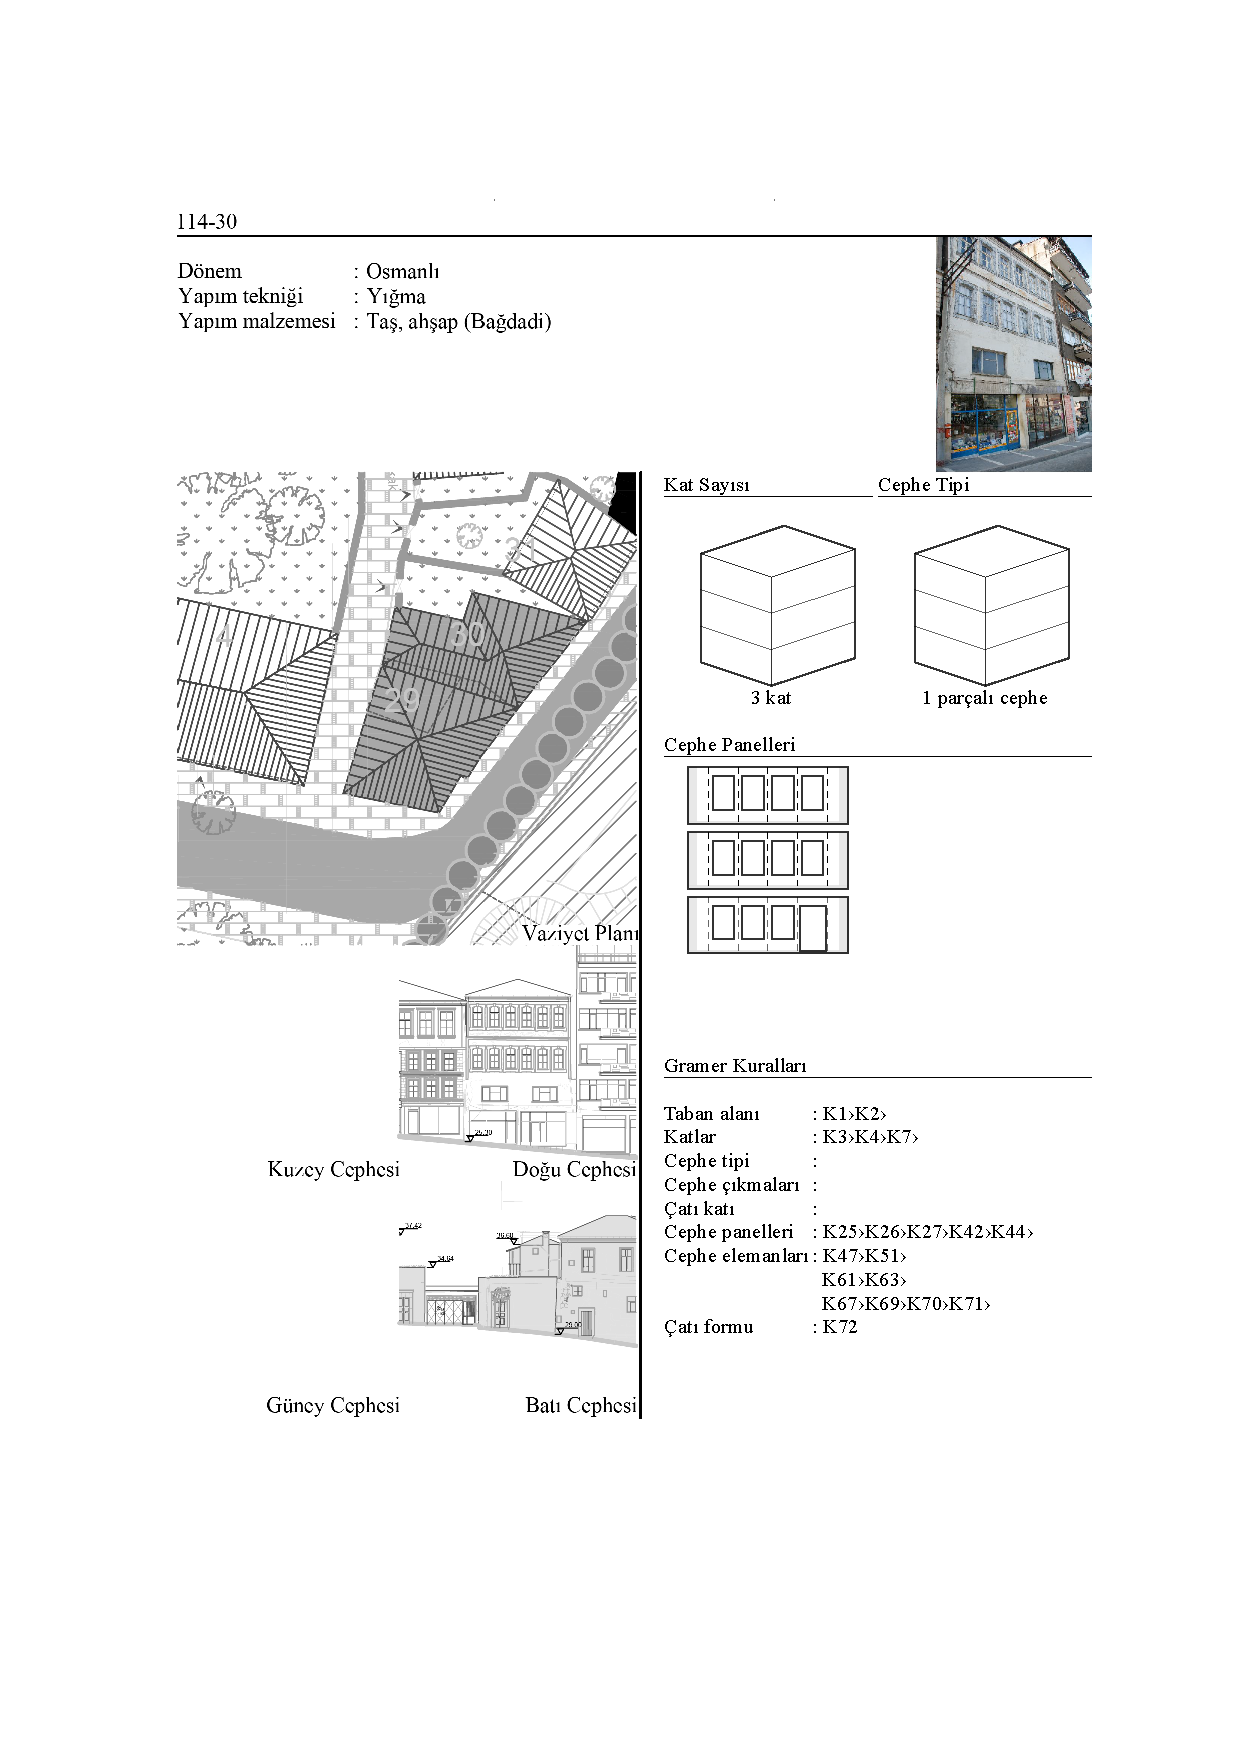
\includegraphics[width=1\textwidth,height=\textheight]{source/figures/BilgiFormlari/114-30.pdf}
\caption{114 ada 30 parsele ait yapı bilgi formu.}
\end{figure}

\begin{figure}
\centering
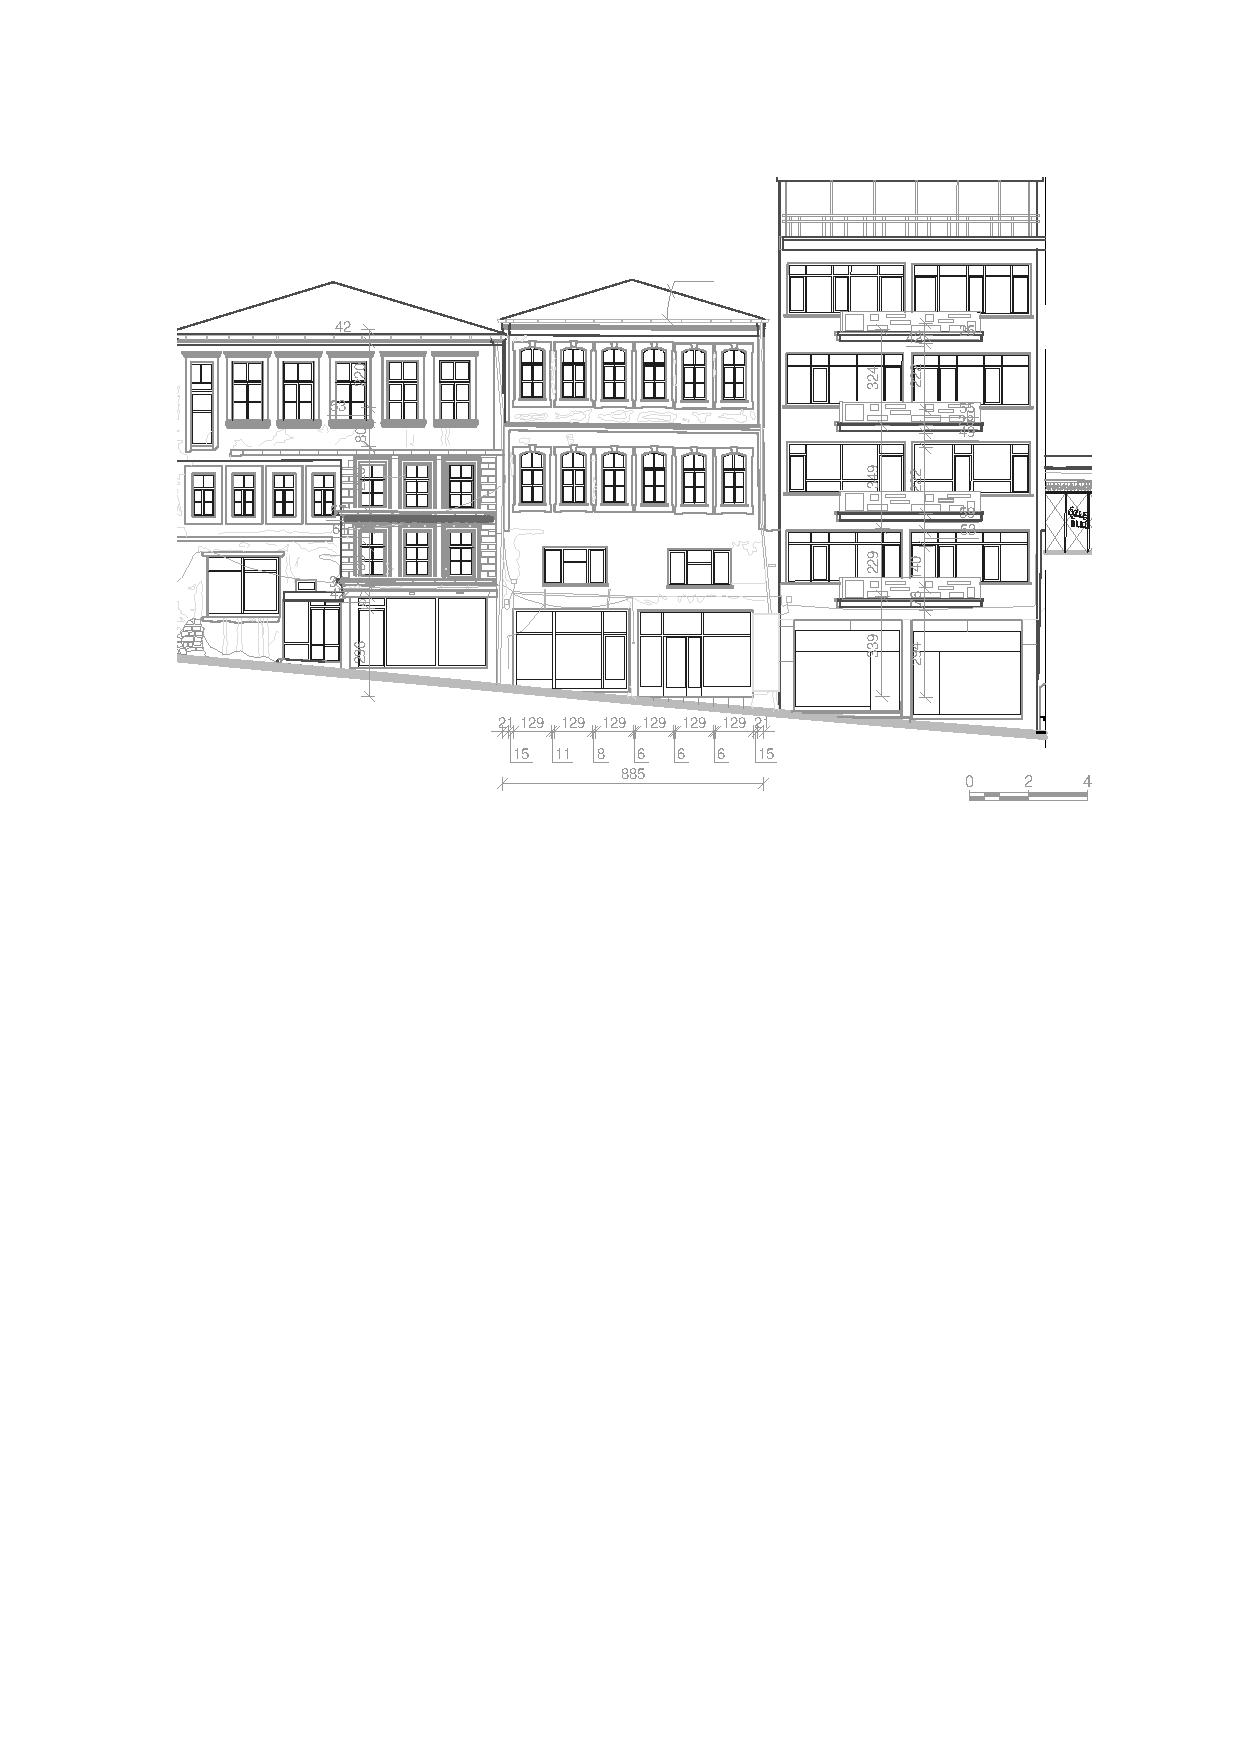
\includegraphics[width=1\textwidth,height=\textheight]{source/figures/Roloveler/R114-30.pdf}
\caption{114 ada 30 parsele ait rölöve çizimi.}
\end{figure}

\begin{figure}
\centering
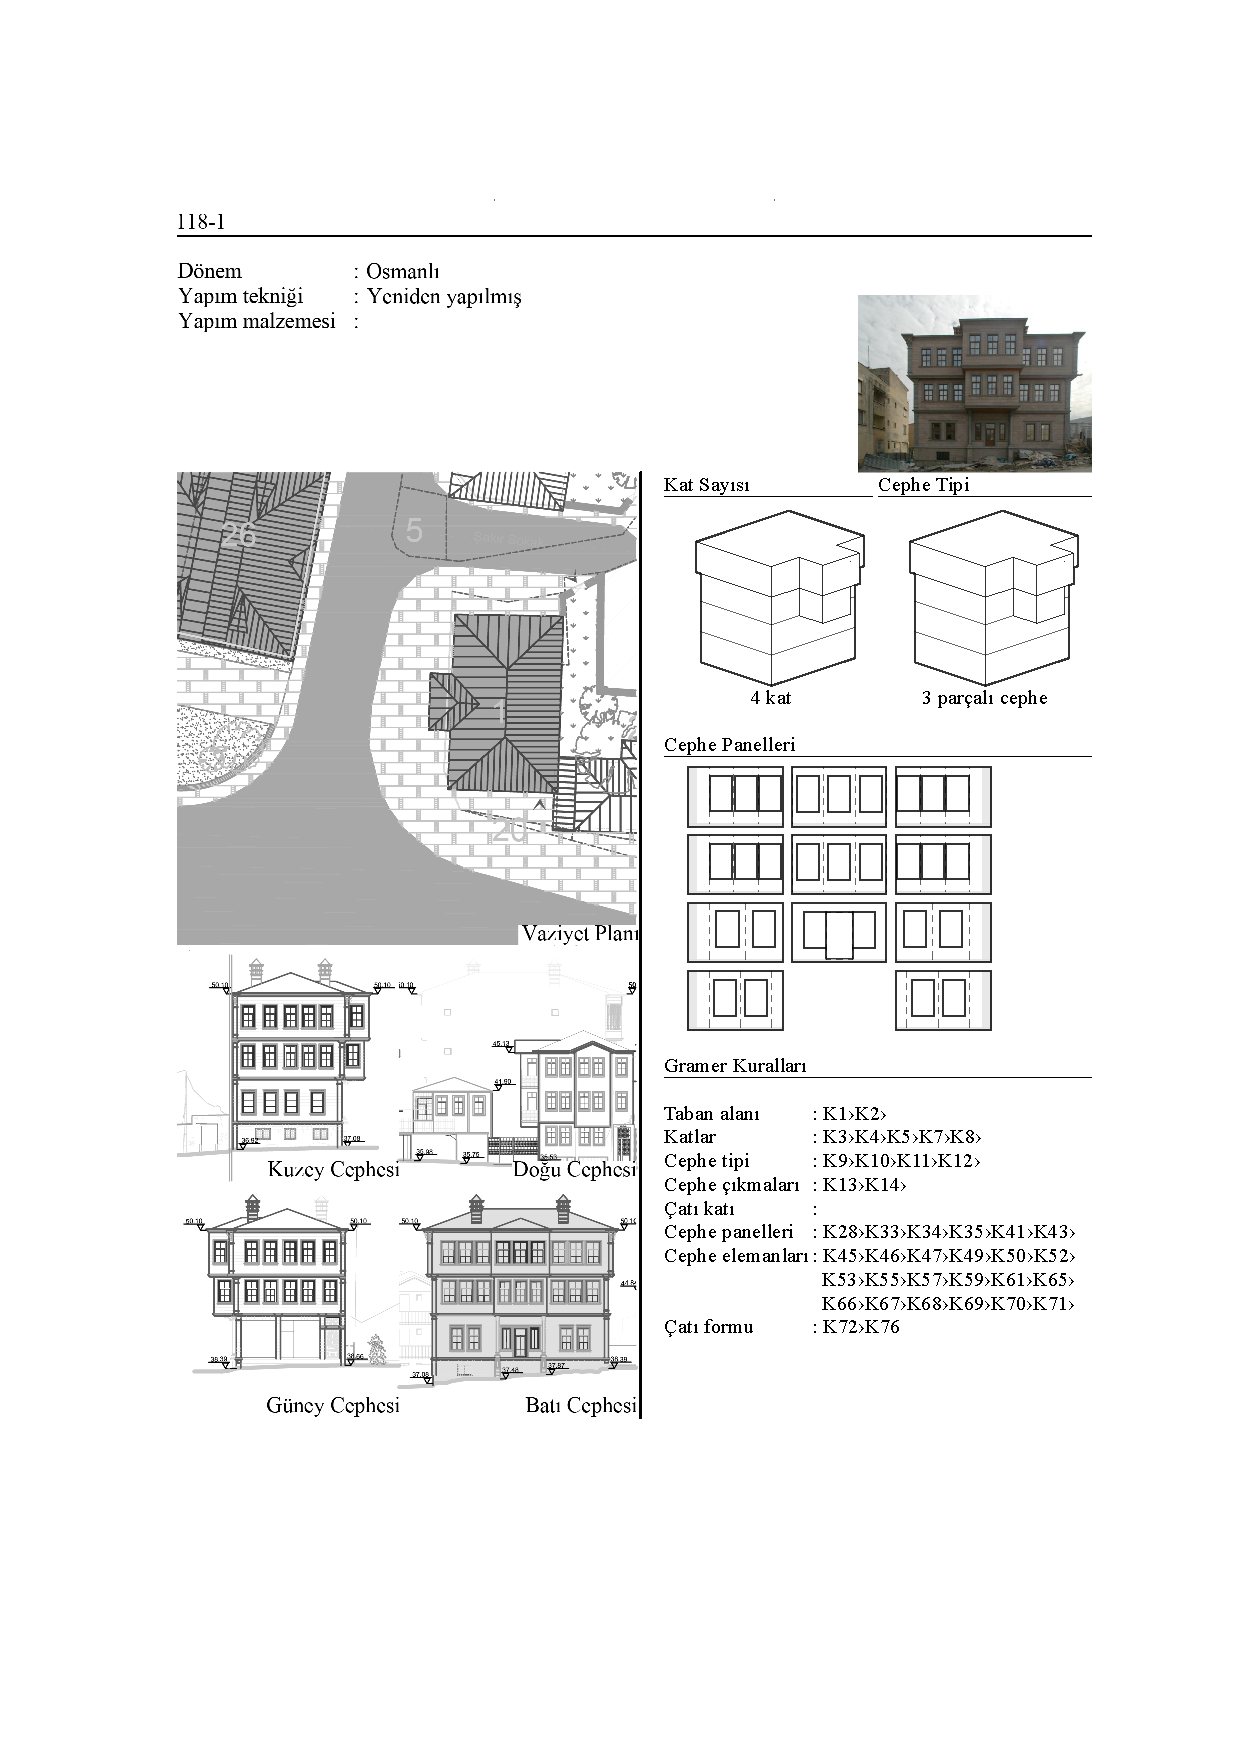
\includegraphics[width=1\textwidth,height=\textheight]{source/figures/BilgiFormlari/118-1.pdf}
\caption{118 ada 1 parsele ait yapı bilgi formu.}
\end{figure}

\begin{figure}
\centering
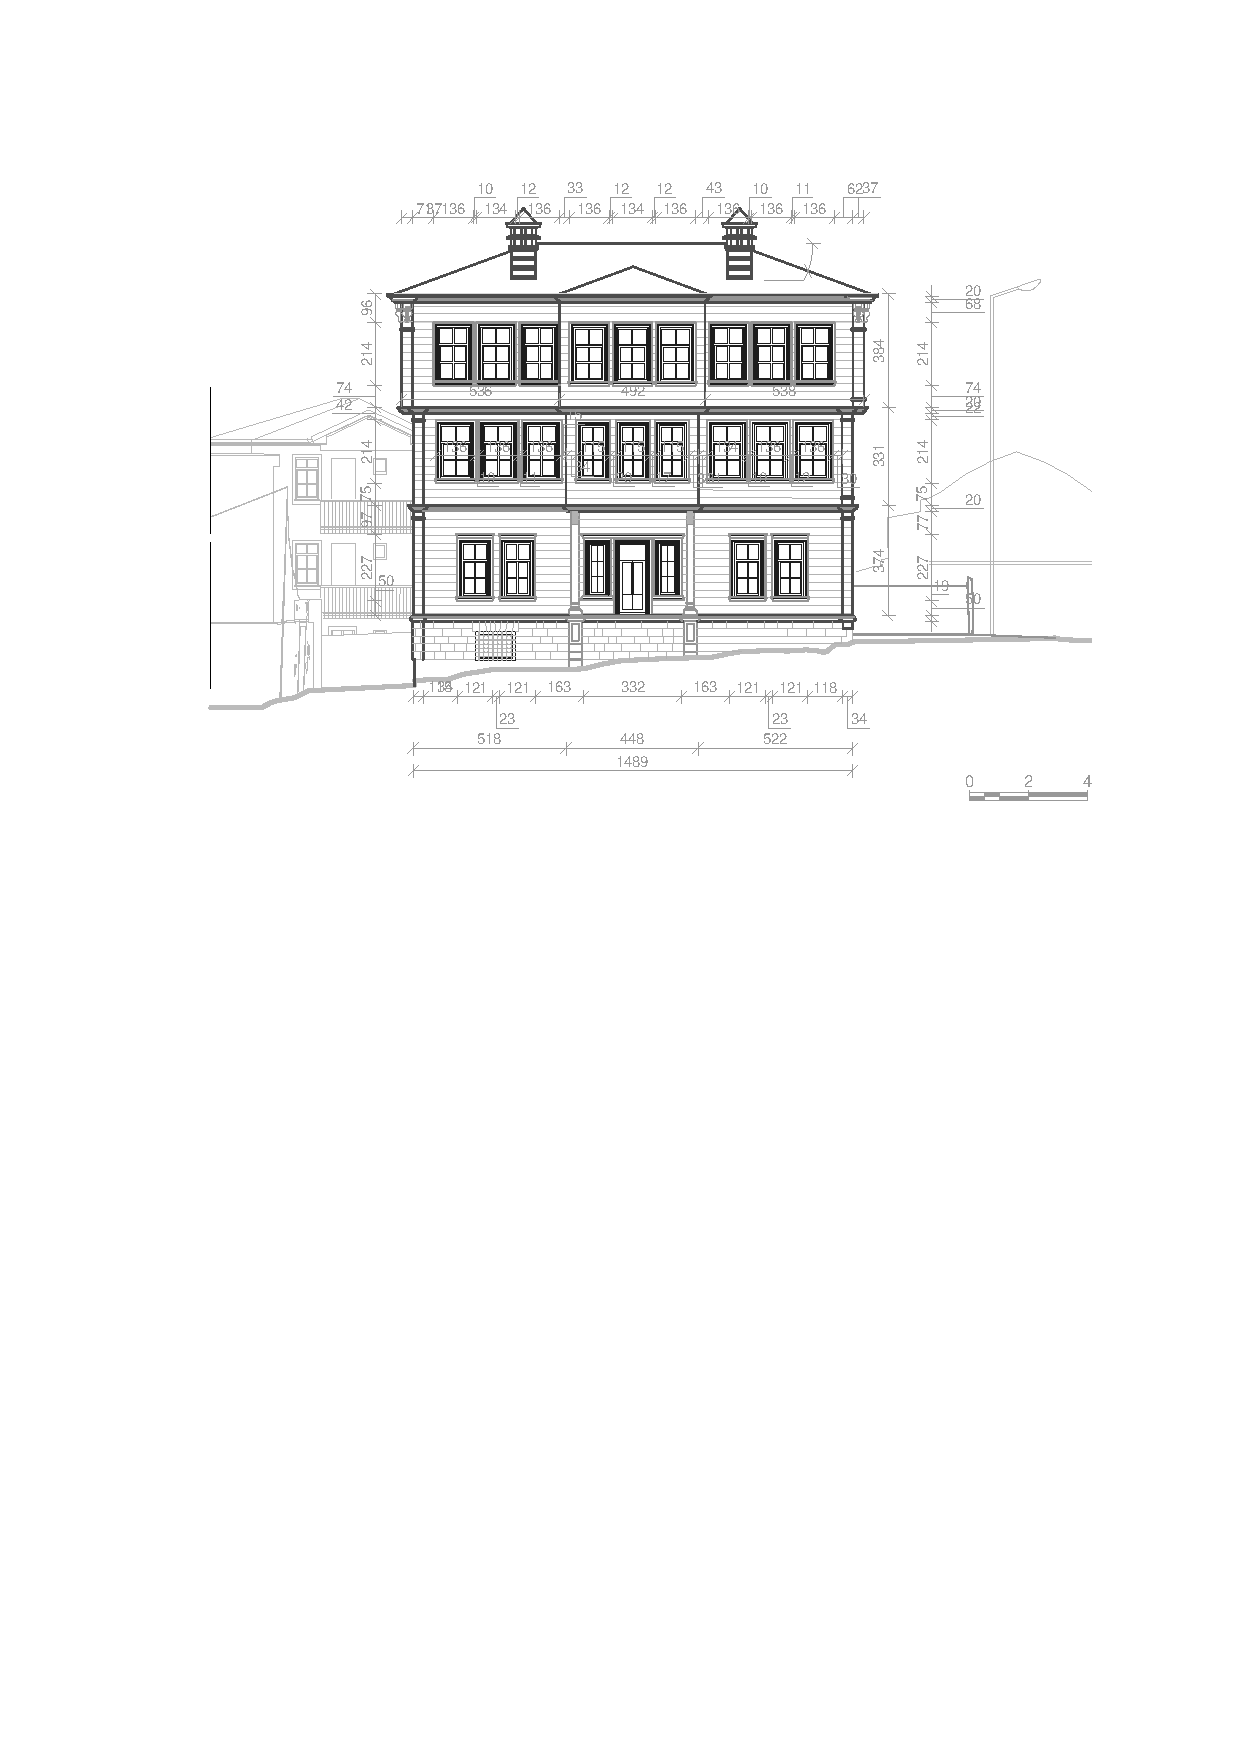
\includegraphics[width=1\textwidth,height=\textheight]{source/figures/Roloveler/R118-1.pdf}
\caption{118 ada 1 parsele ait rölöve çizimi.}
\end{figure}

\begin{figure}
\centering
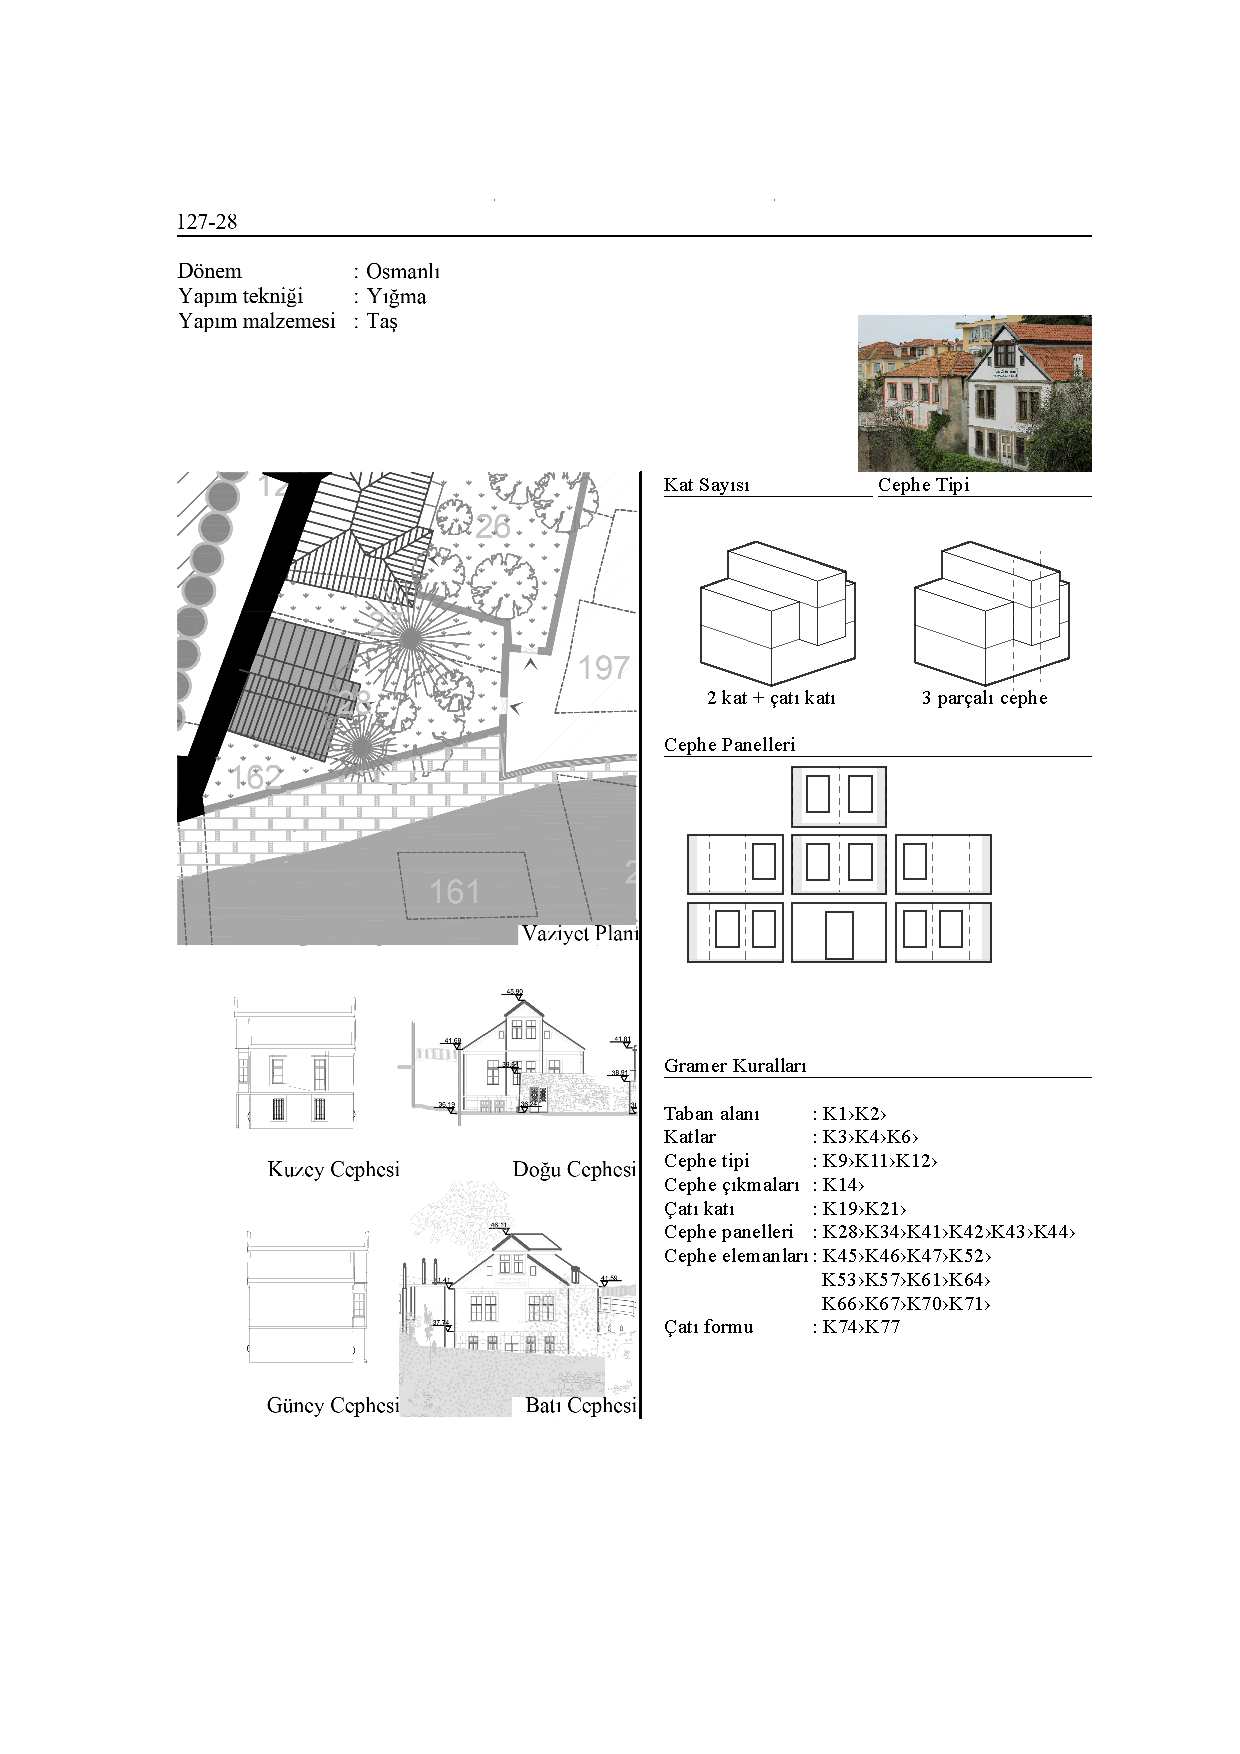
\includegraphics[width=1\textwidth,height=\textheight]{source/figures/BilgiFormlari/127-28.pdf}
\caption{127 ada 28 parsele ait yapı bilgi formu.}
\end{figure}

\begin{figure}
\centering
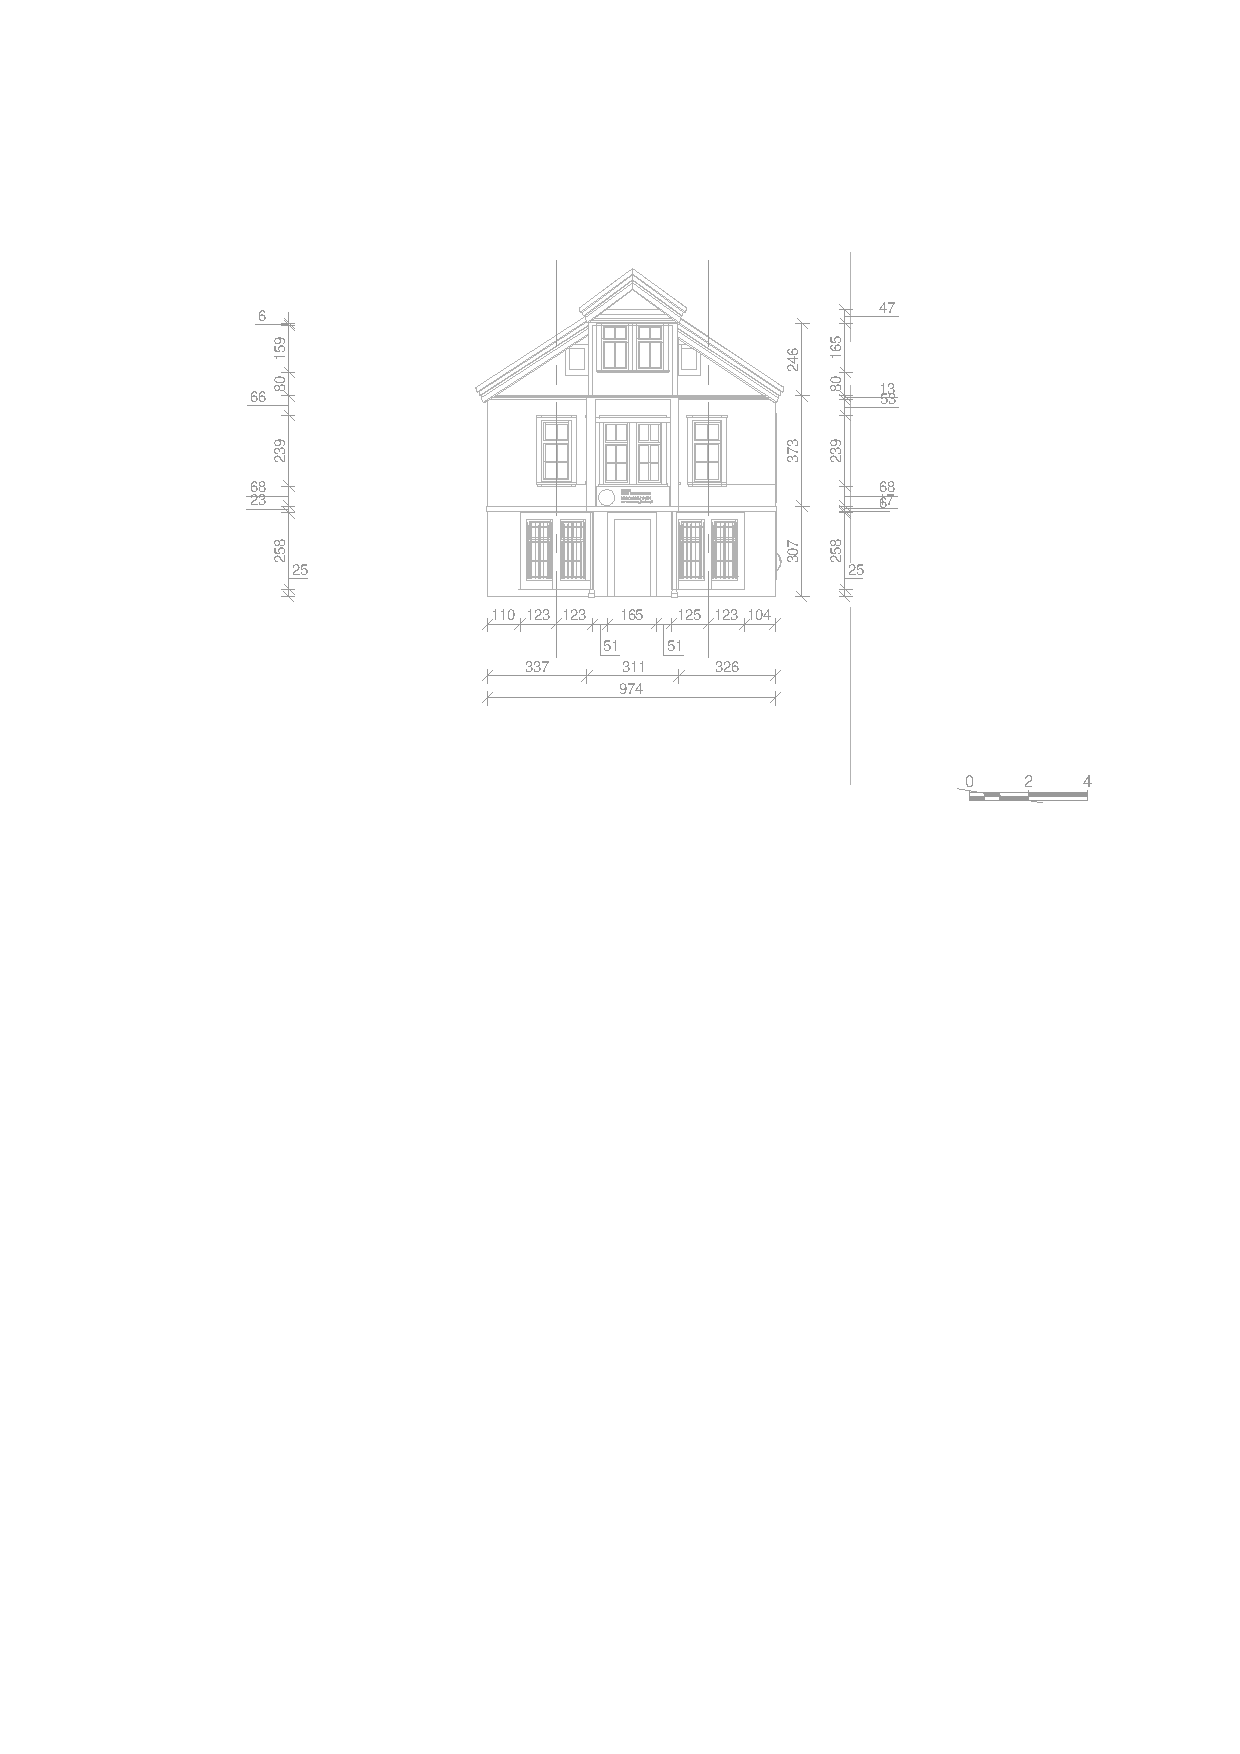
\includegraphics[width=1\textwidth,height=\textheight]{source/figures/Roloveler/R127-28.pdf}
\caption{127 ada 28 parsele ait rölöve çizimi.}
\end{figure}

\begin{figure}
\centering
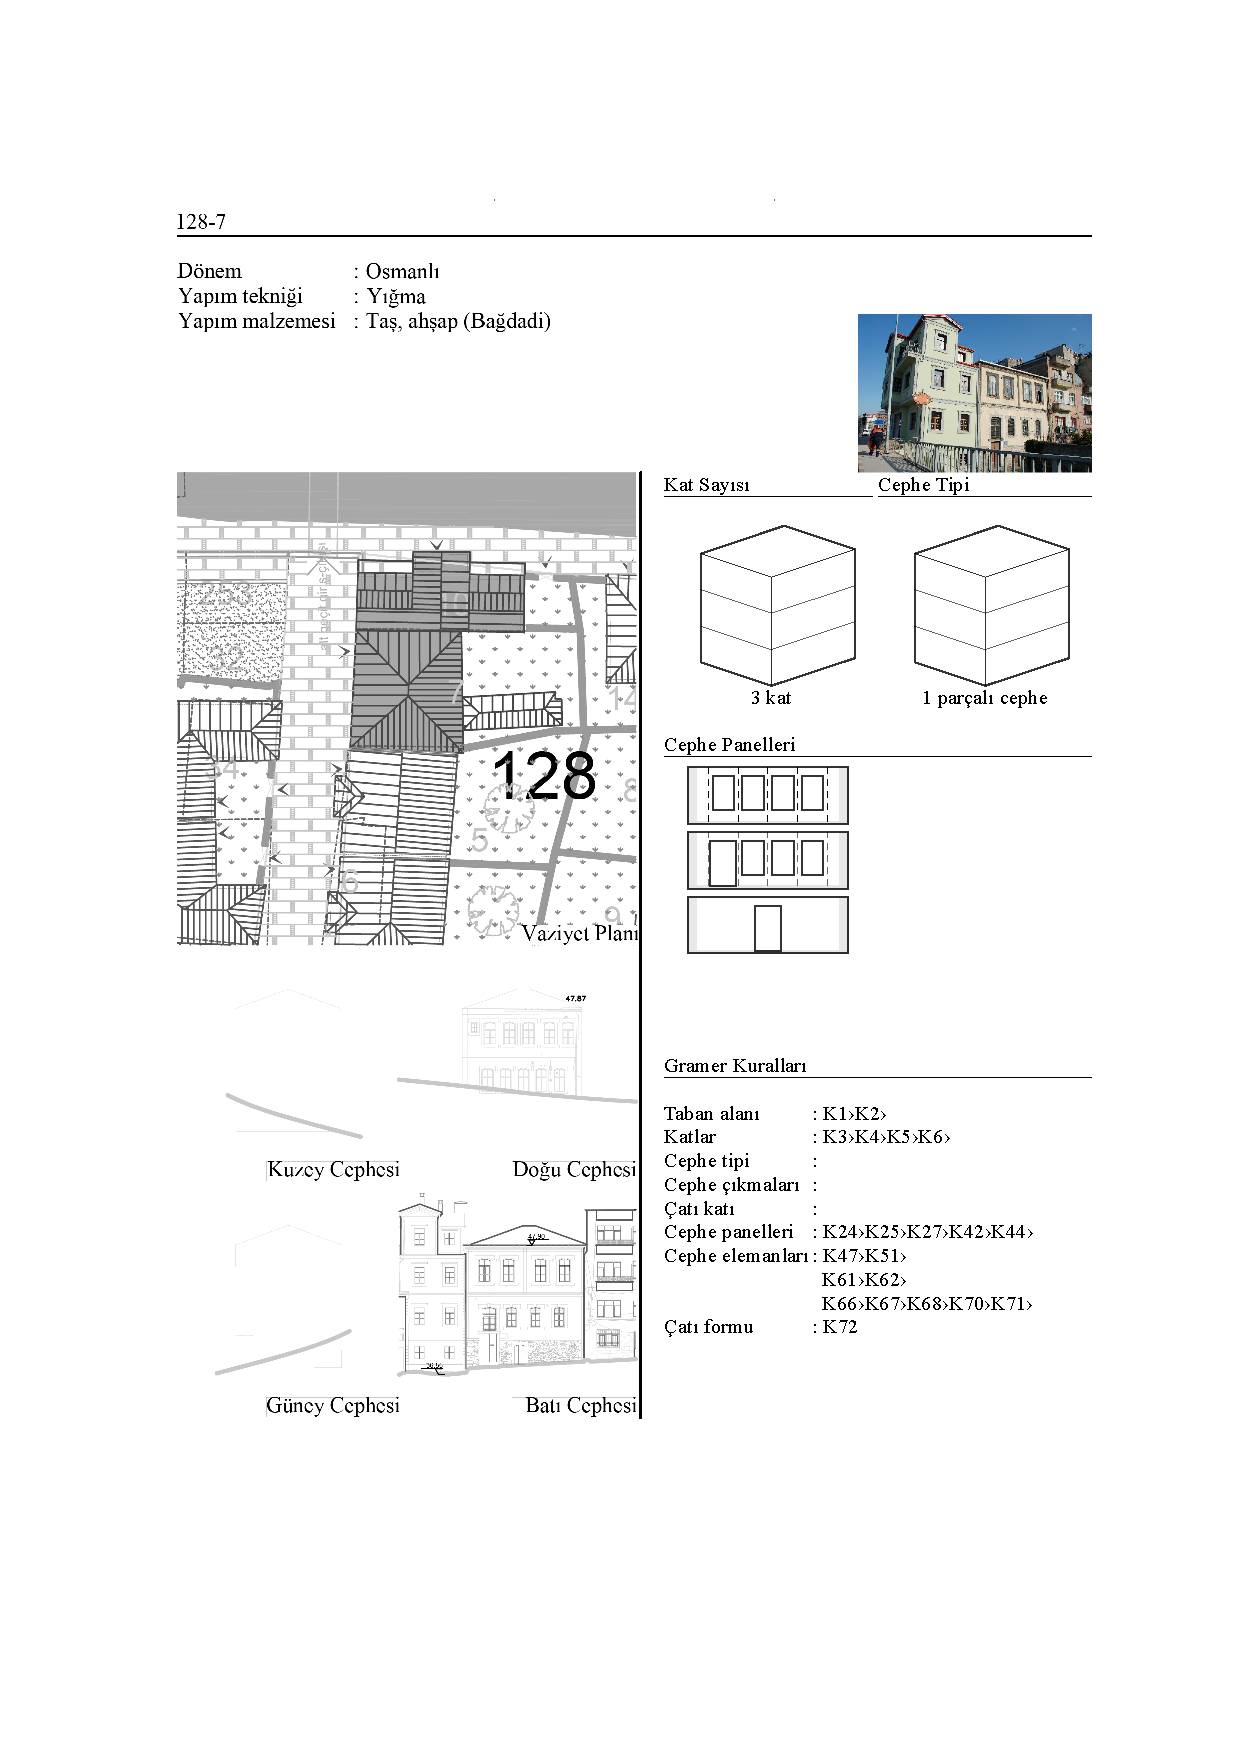
\includegraphics[width=1\textwidth,height=\textheight]{source/figures/BilgiFormlari/128-7.pdf}
\caption{128 ada 7 parsele ait yapı bilgi formu.}
\end{figure}

\begin{figure}
\centering
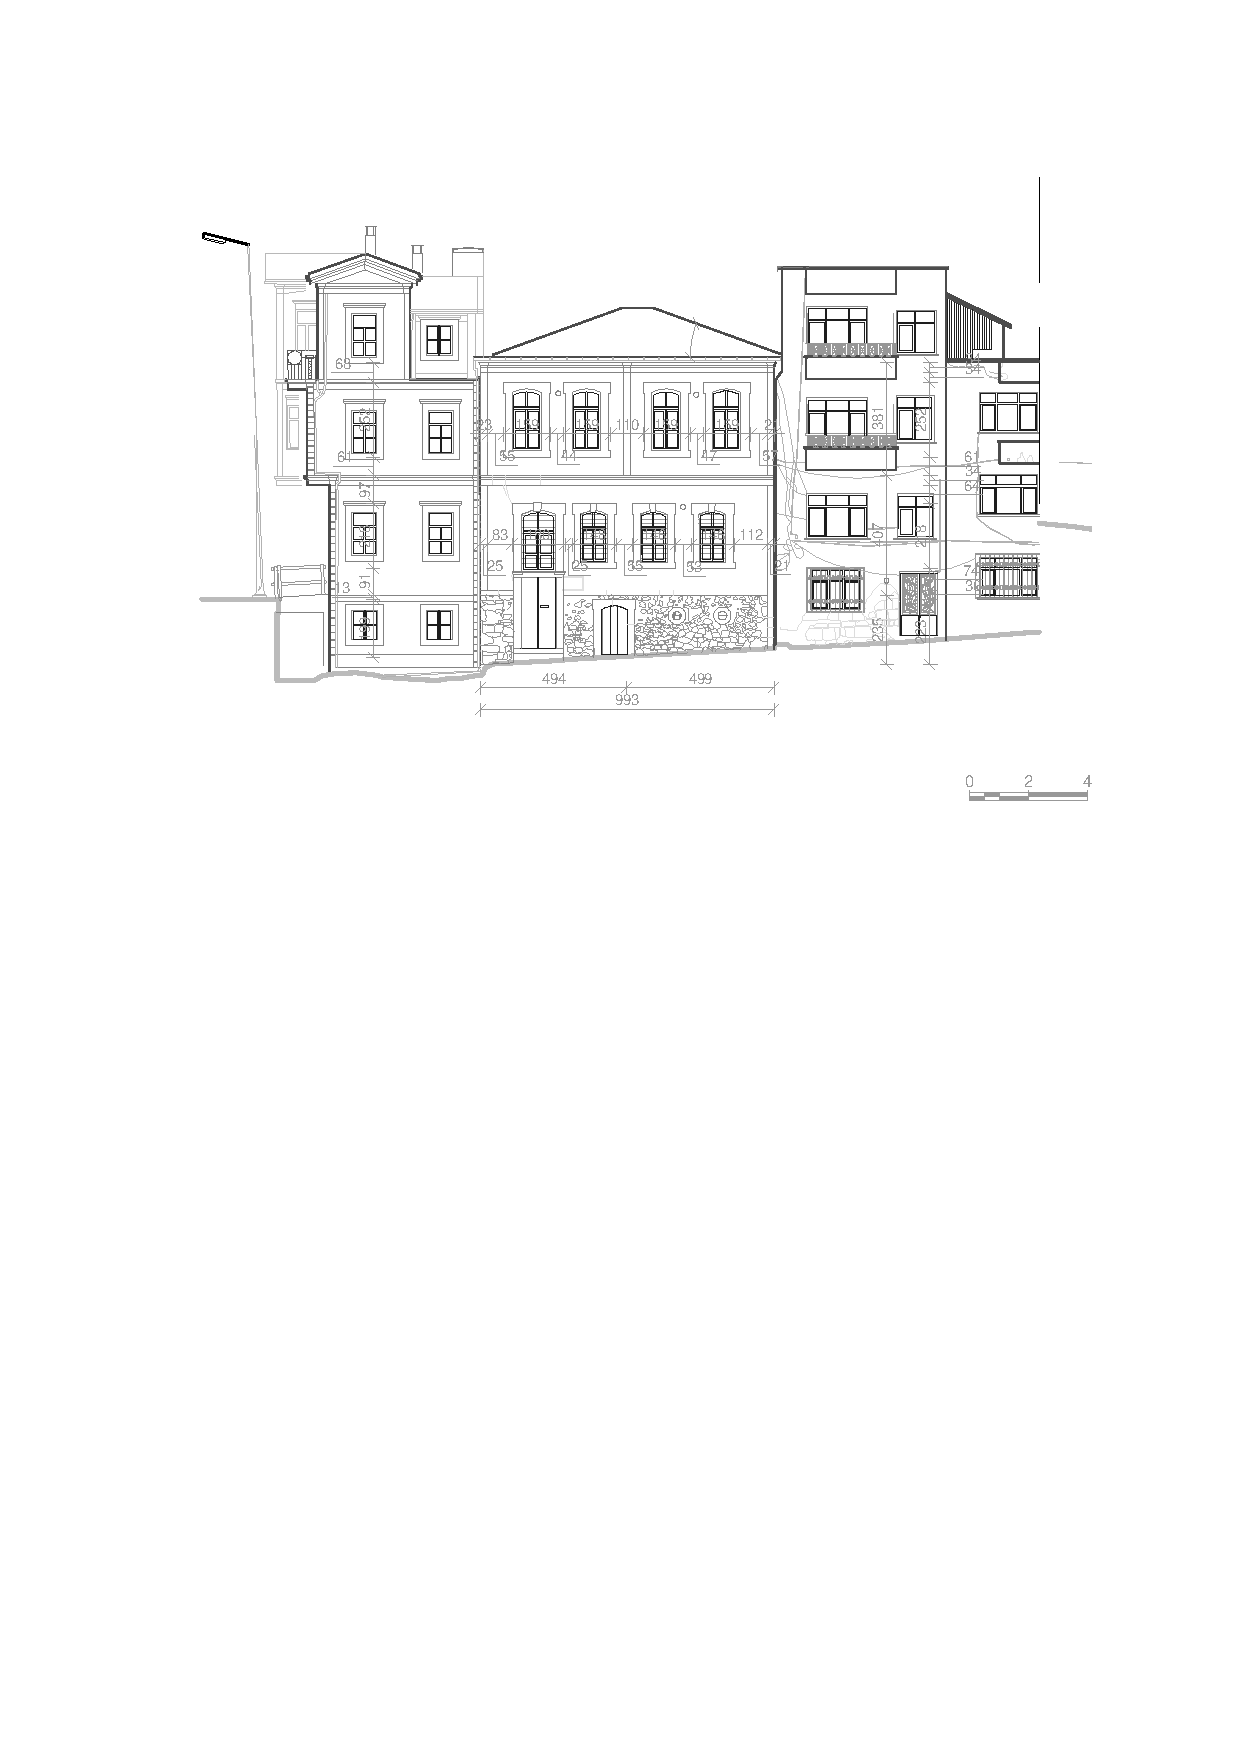
\includegraphics[width=1\textwidth,height=\textheight]{source/figures/Roloveler/R128-7.pdf}
\caption{128 ada 7 parsele ait rölöve çizimi.}
\end{figure}

\begin{figure}
\centering
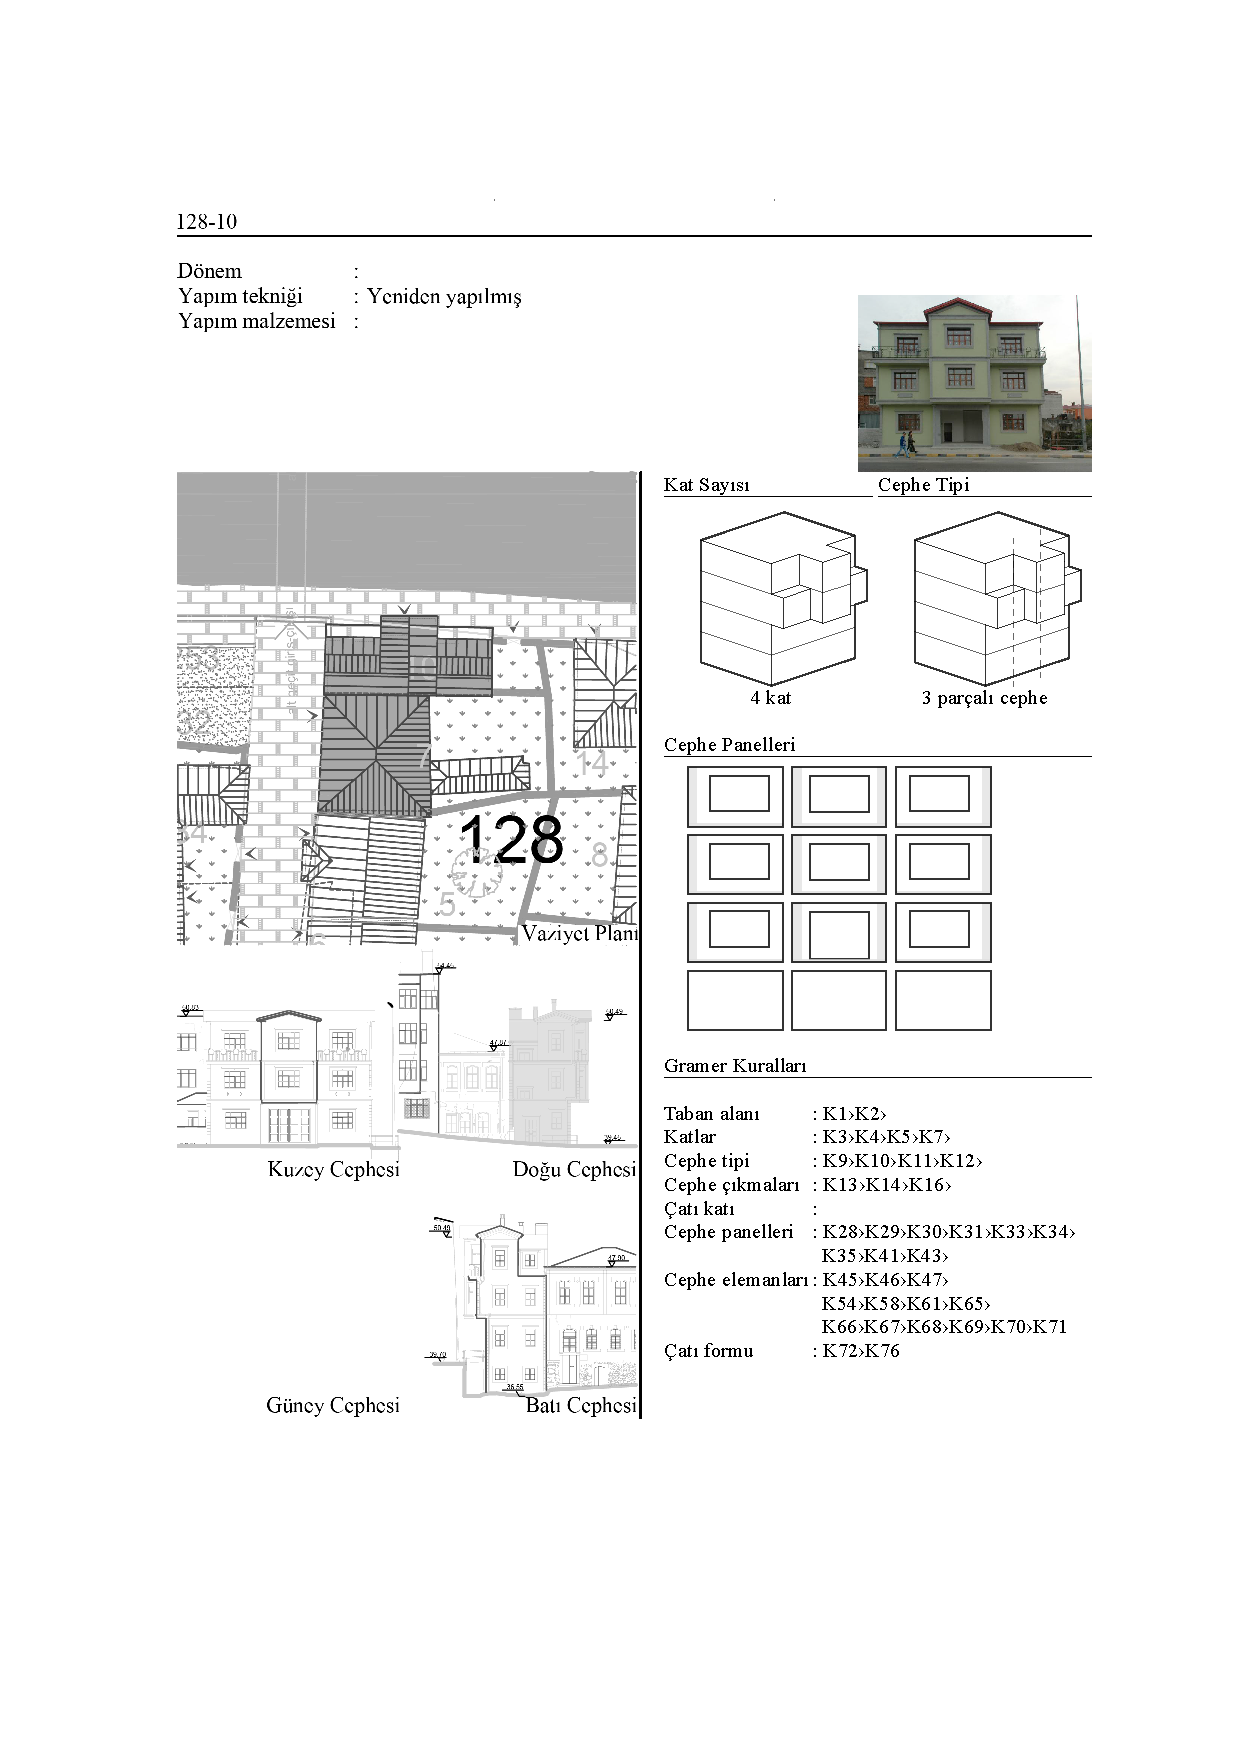
\includegraphics[width=1\textwidth,height=\textheight]{source/figures/BilgiFormlari/128-10.pdf}
\caption{128 ada 10 parsele ait yapı bilgi formu.}
\end{figure}

\begin{figure}
\centering
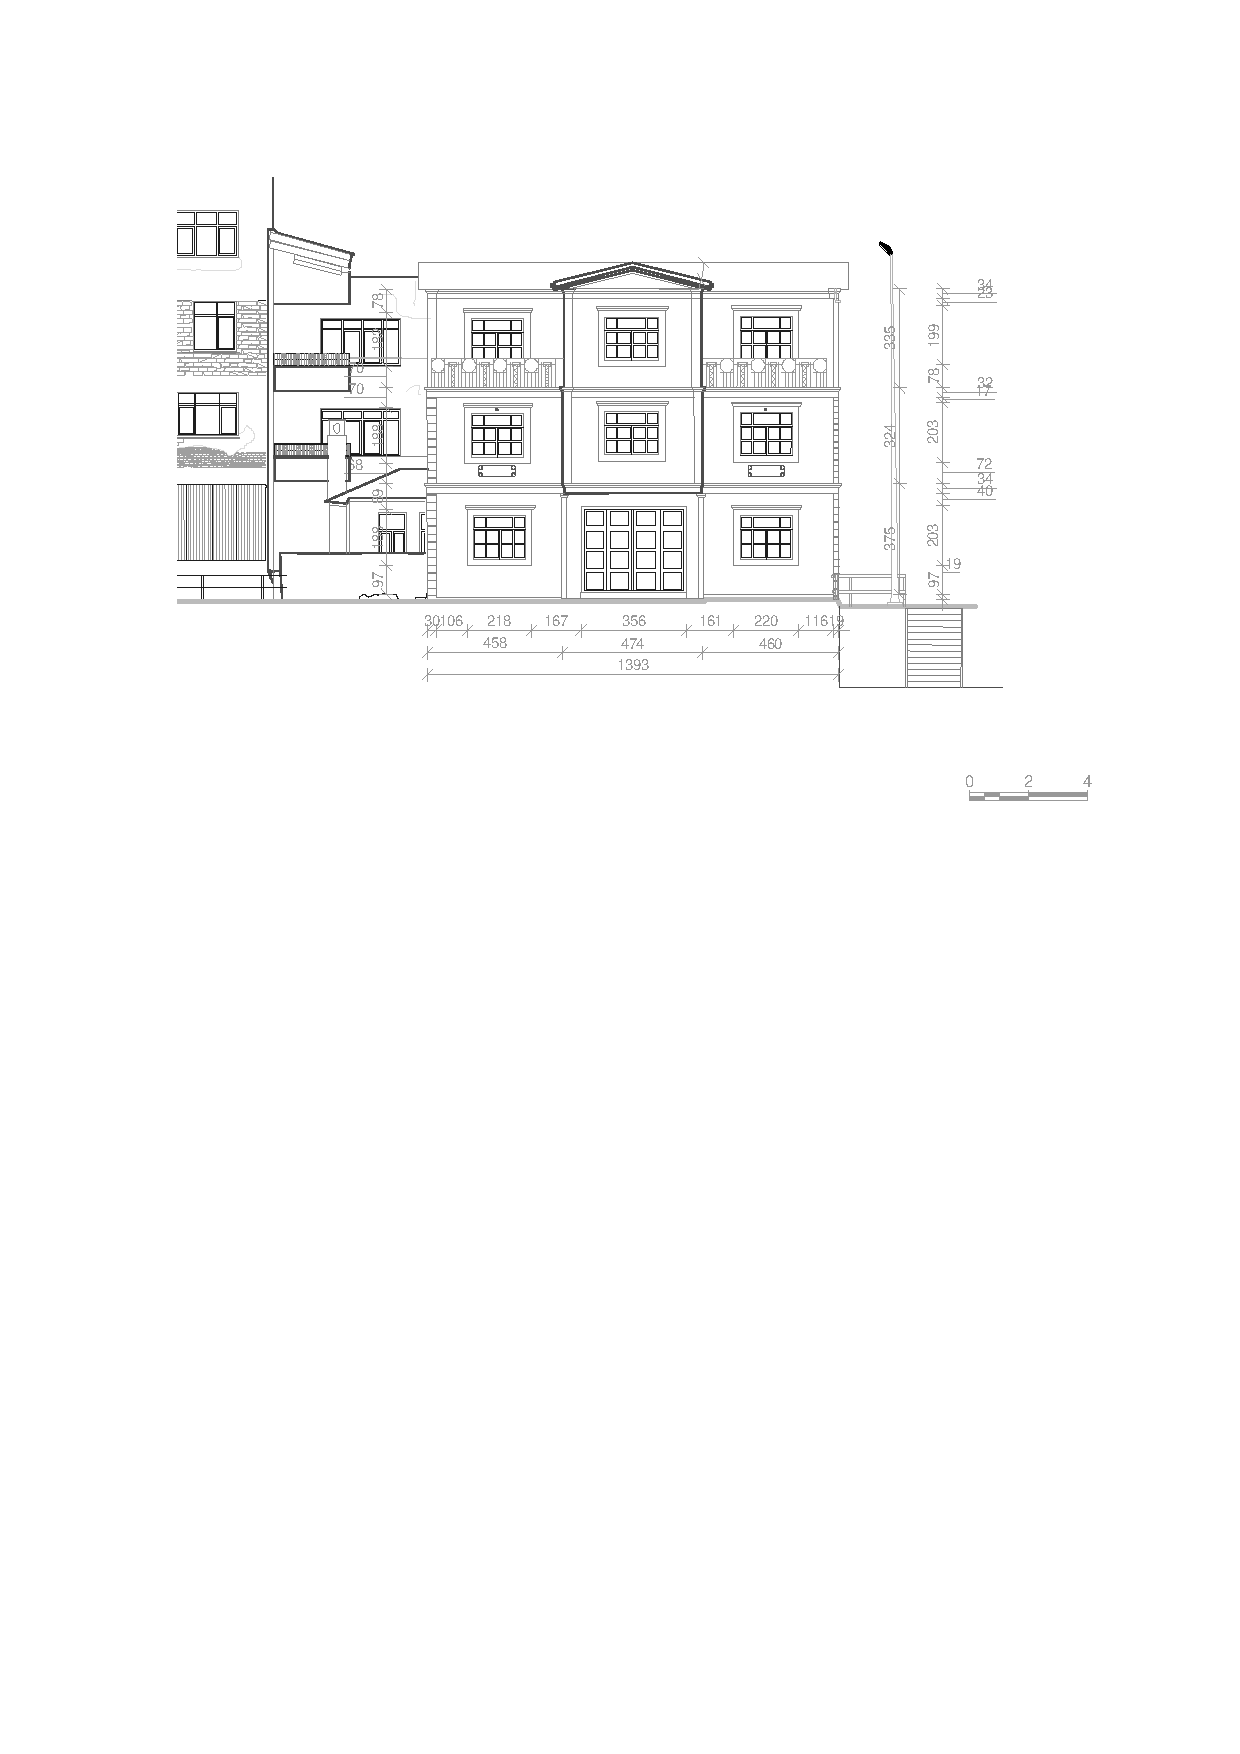
\includegraphics[width=1\textwidth,height=\textheight]{source/figures/Roloveler/R128-10.pdf}
\caption{128 ada 10 parsele ait rölöve çizimi.}
\end{figure}

\begin{figure}
\centering
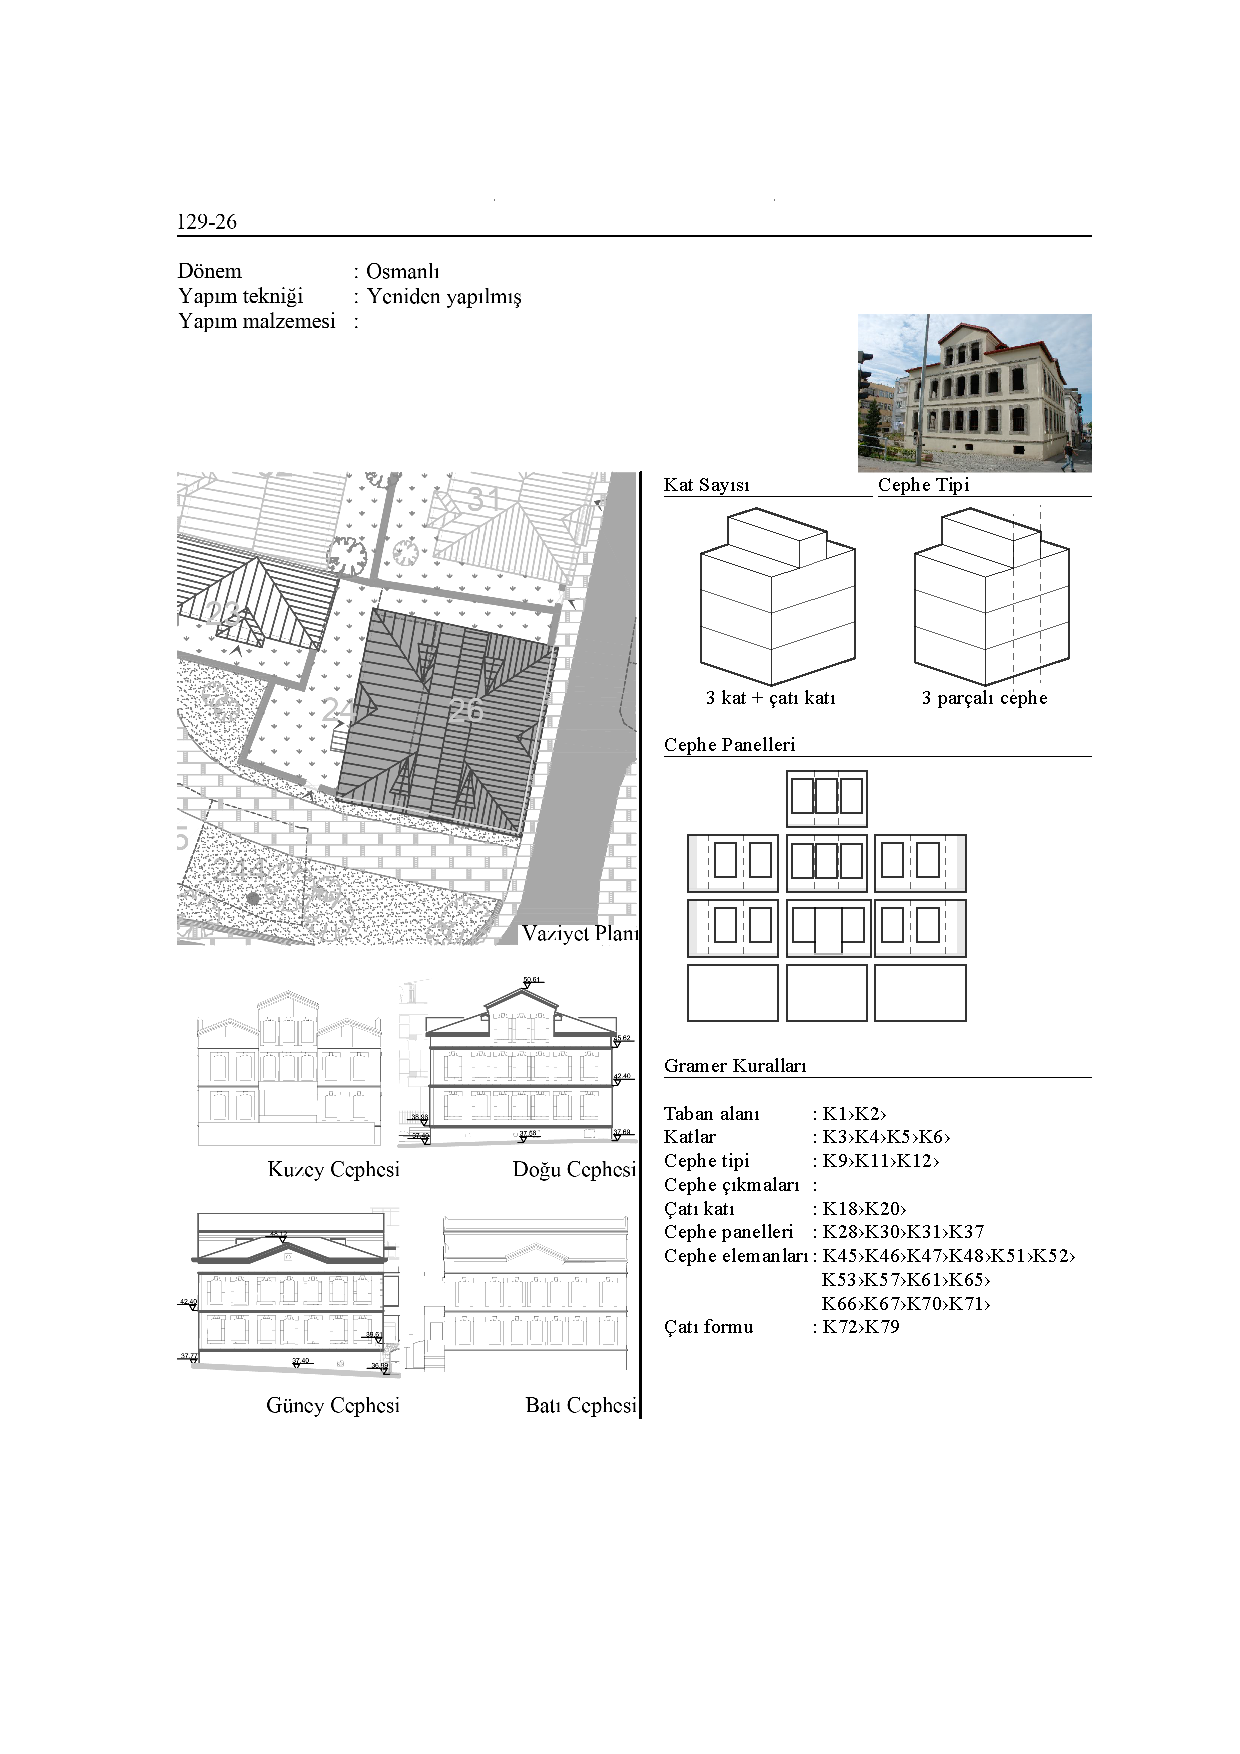
\includegraphics[width=1\textwidth,height=\textheight]{source/figures/BilgiFormlari/129-26.pdf}
\caption{129 ada 26 parsele ait yapı bilgi formu.}
\end{figure}

\begin{figure}
\centering
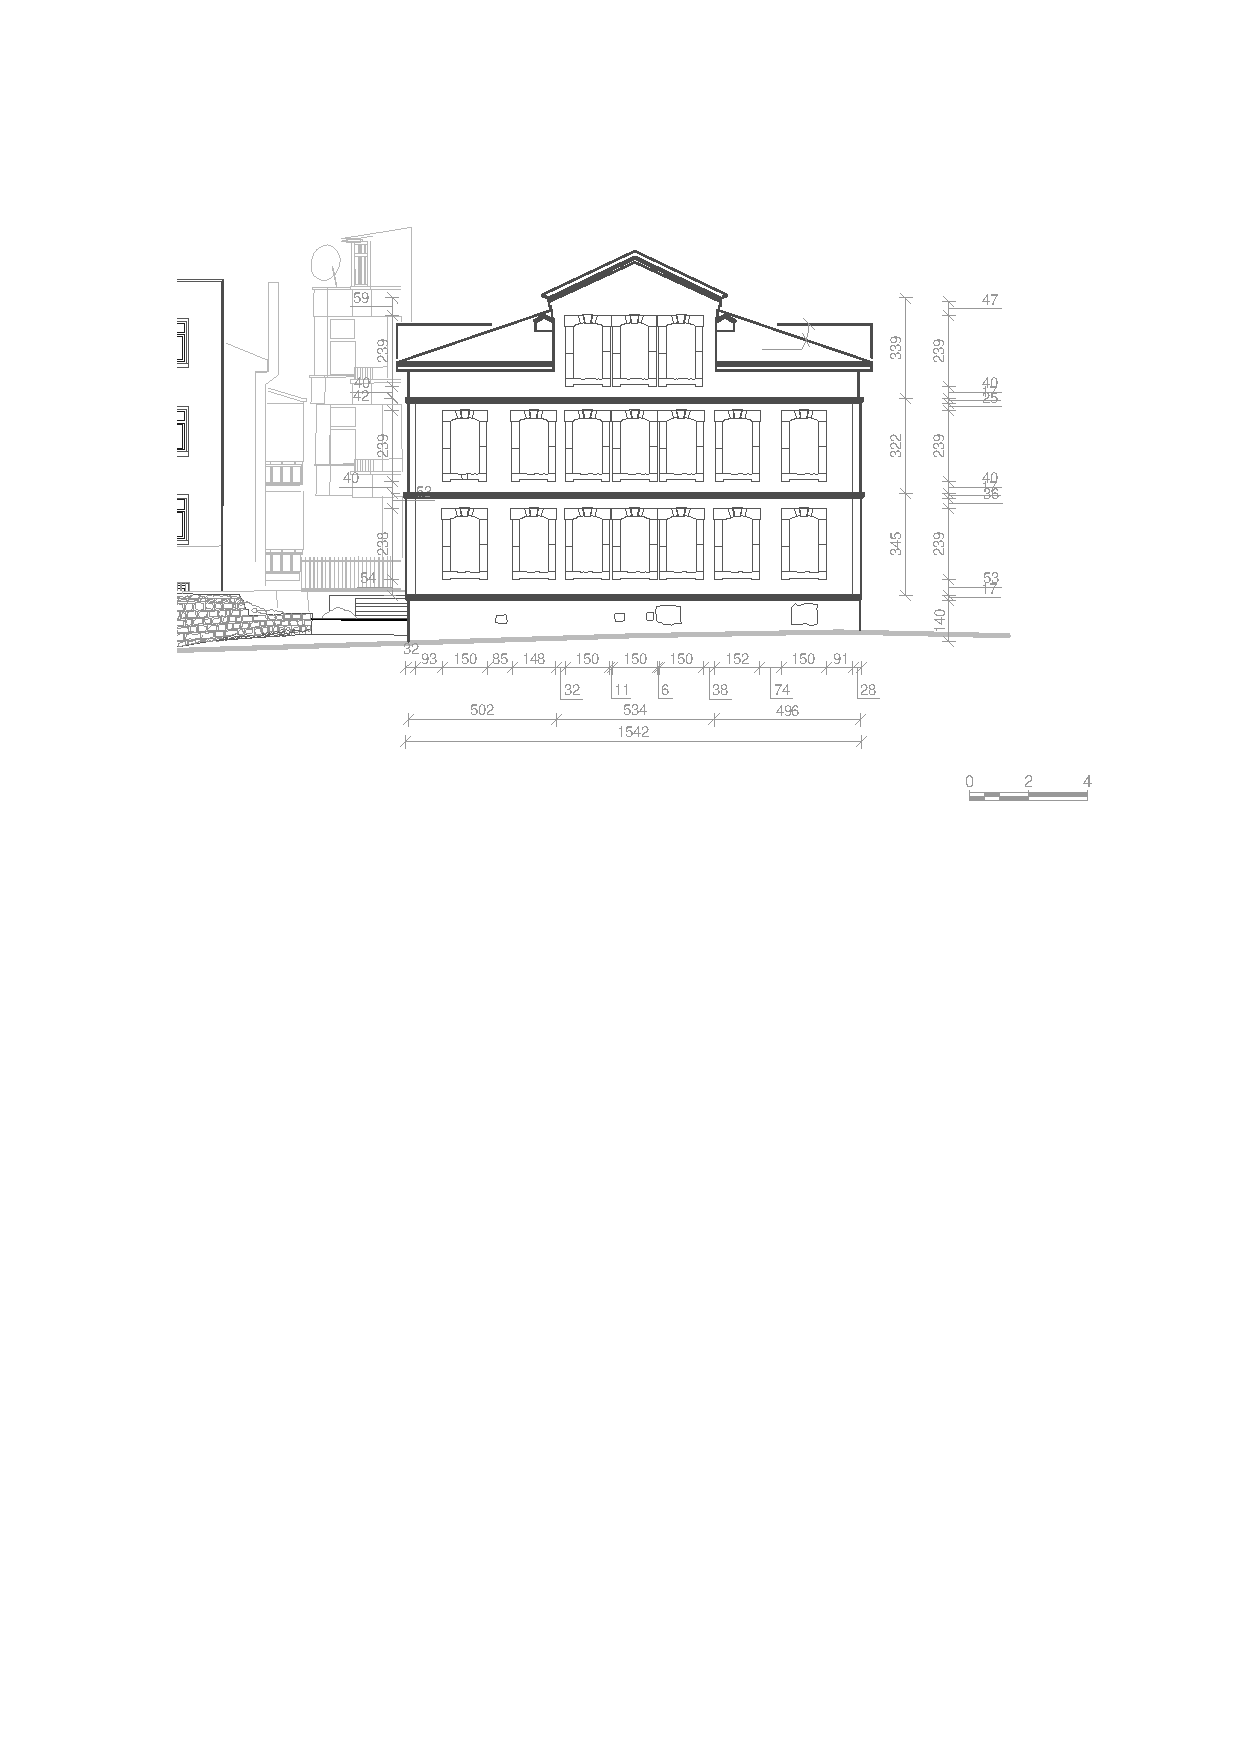
\includegraphics[width=1\textwidth,height=\textheight]{source/figures/Roloveler/R129-26.pdf}
\caption{129 ada 26 parsele ait rölöve çizimi.}
\end{figure}

\begin{figure}
\centering
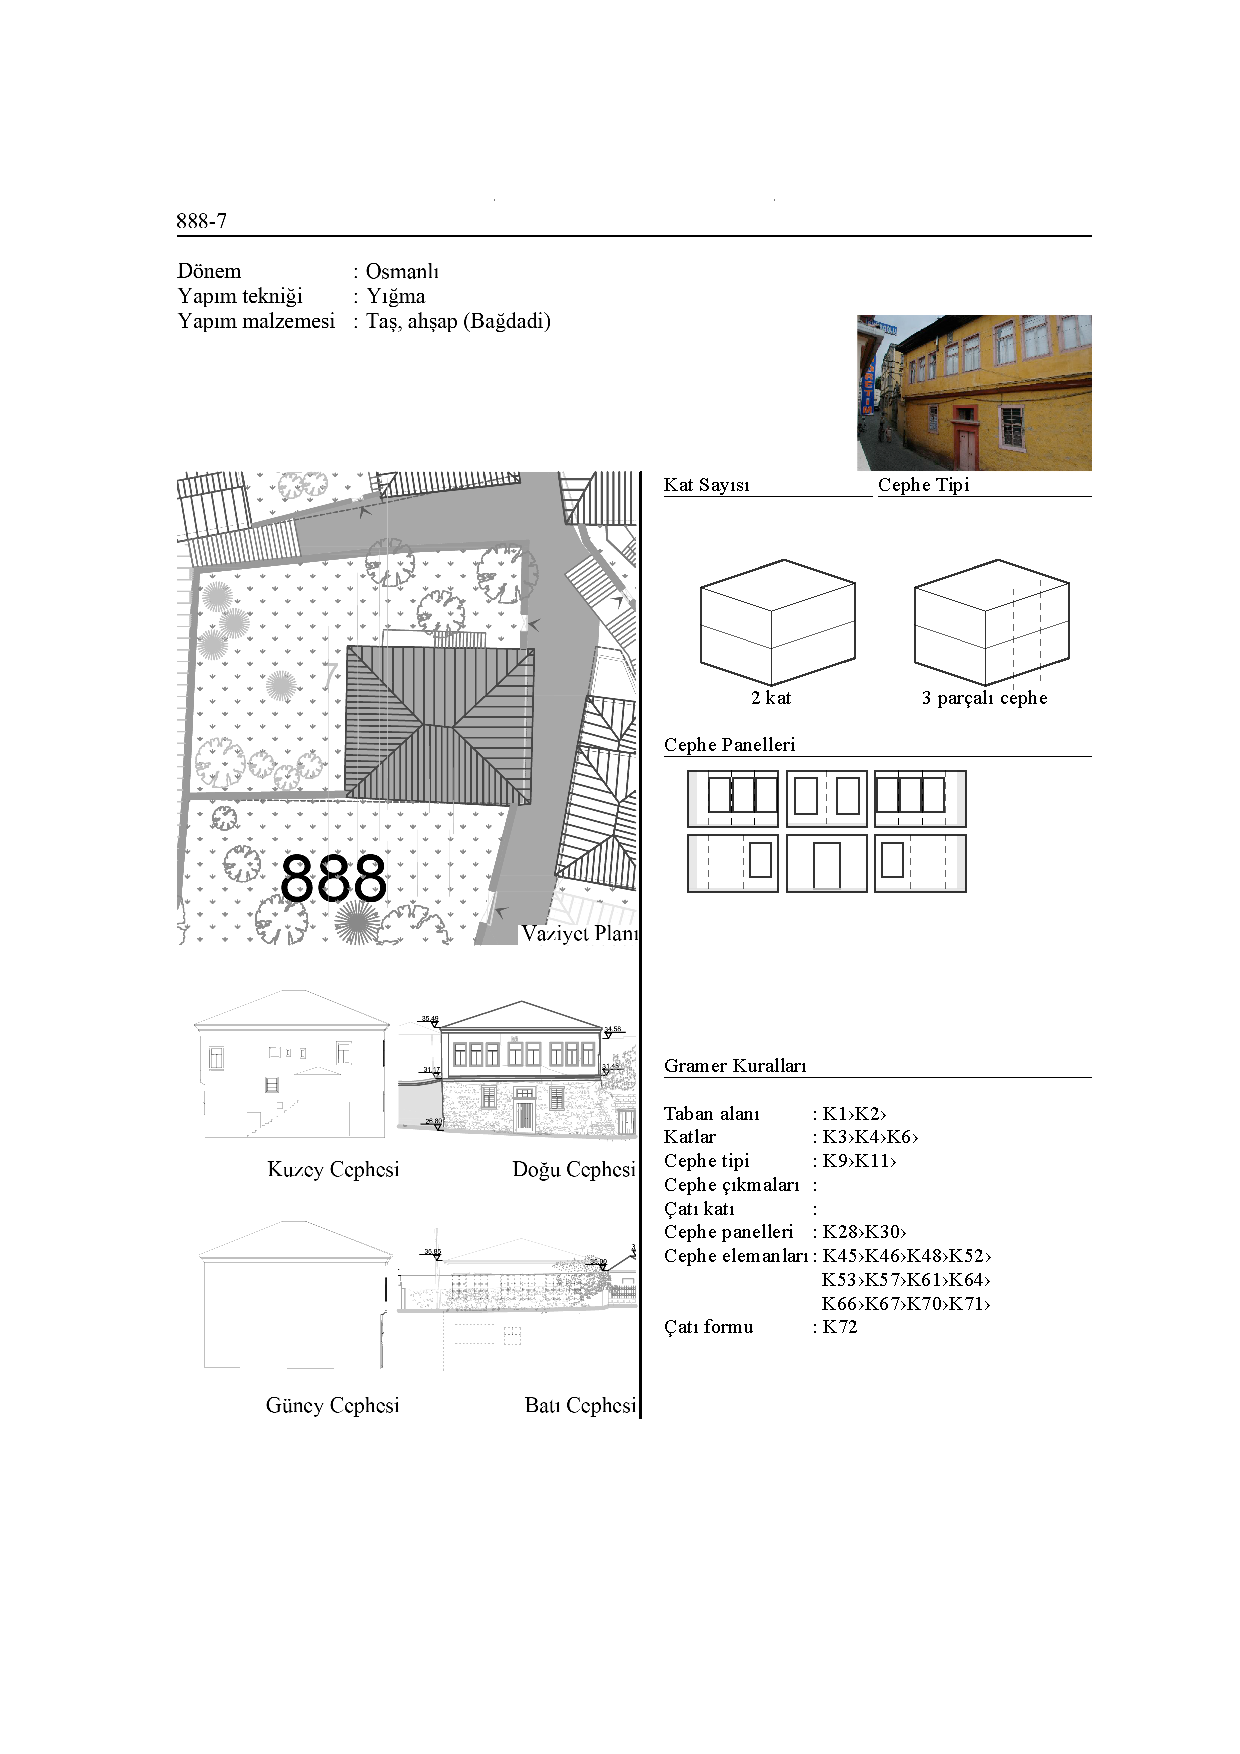
\includegraphics[width=1\textwidth,height=\textheight]{source/figures/BilgiFormlari/888-7.pdf}
\caption{888 ada 7 parsele ait yapı bilgi formu.}
\end{figure}

\begin{figure}
\centering
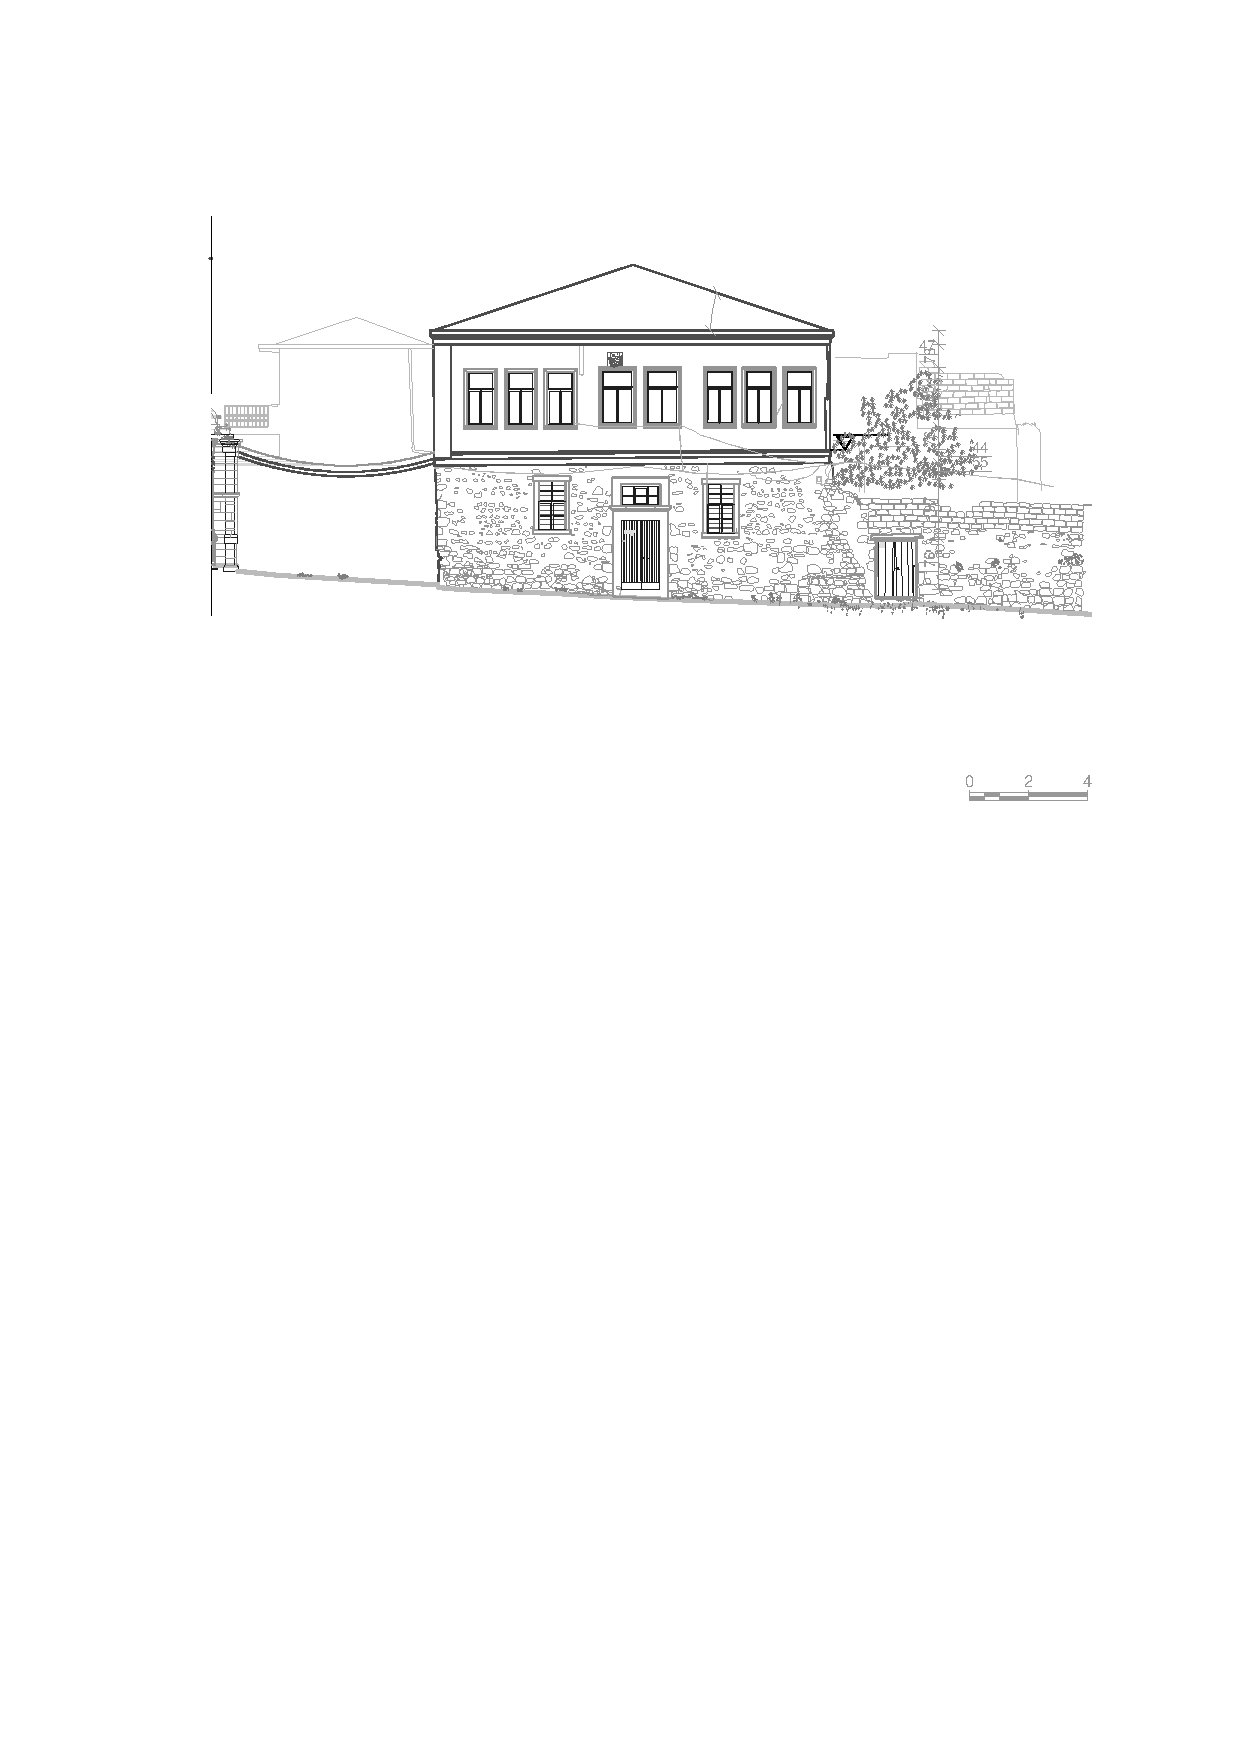
\includegraphics[width=1\textwidth,height=\textheight]{source/figures/Roloveler/R888-7.pdf}
\caption{888 ada 7 parsele ait rölöve çizimi.}
\end{figure}

\begin{figure}
\centering
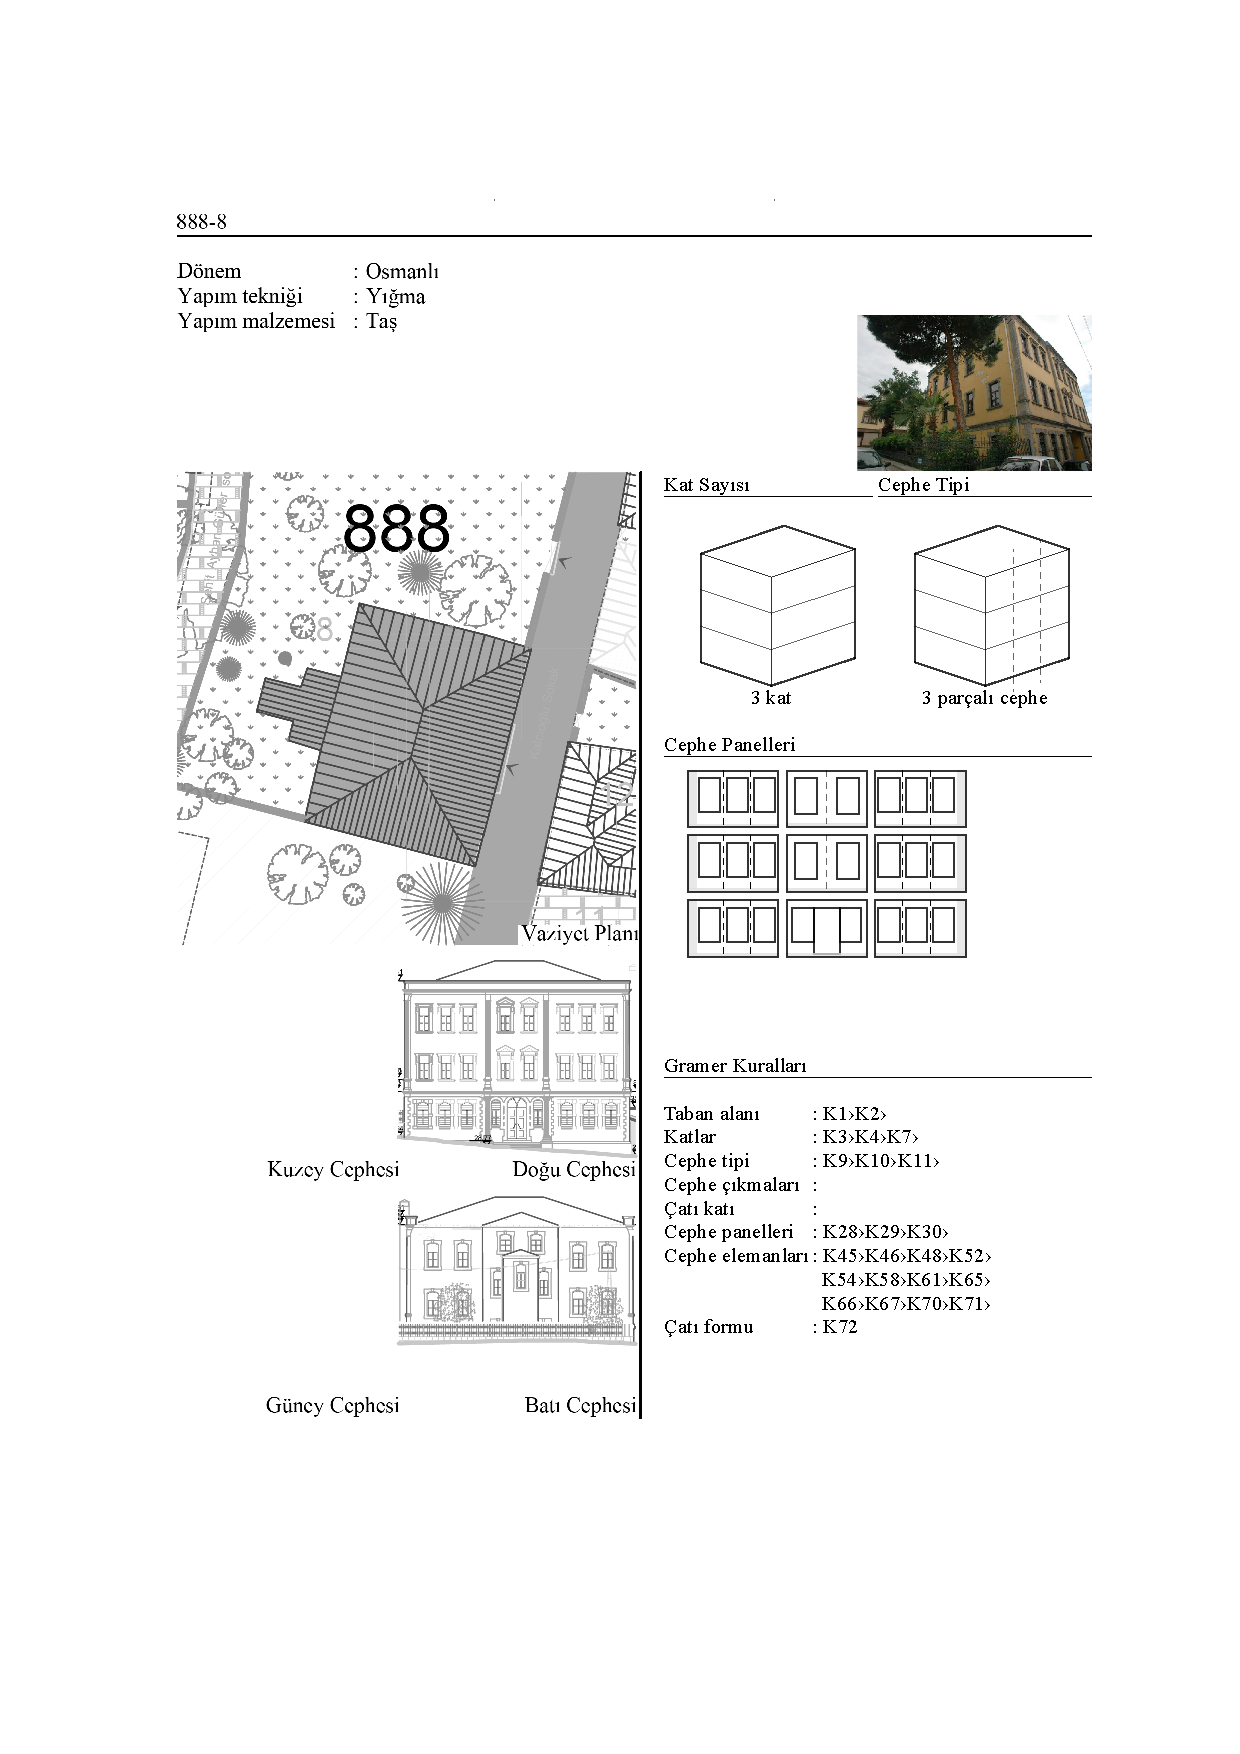
\includegraphics[width=1\textwidth,height=\textheight]{source/figures/BilgiFormlari/888-8.pdf}
\caption{888 ada 8 parsele ait yapı bilgi formu.}
\end{figure}

\begin{figure}
\centering
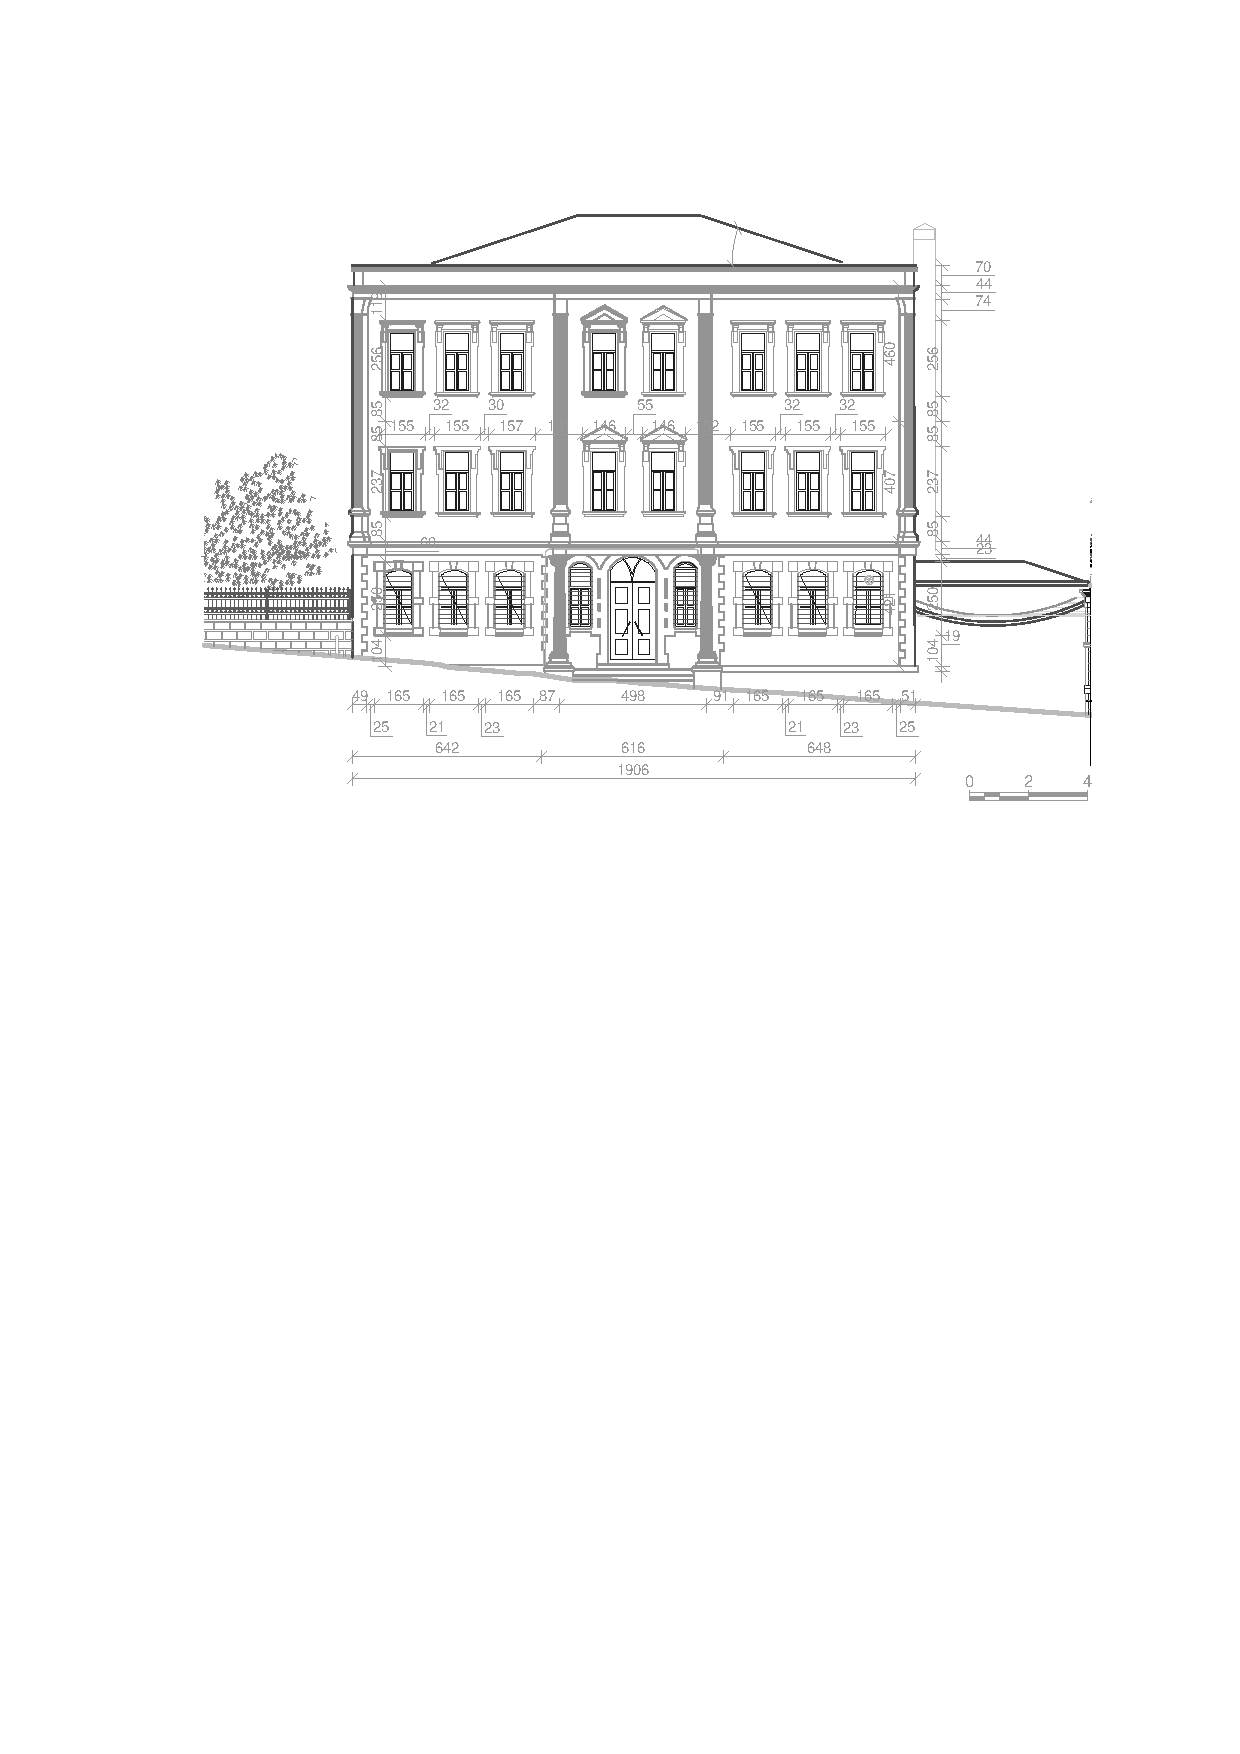
\includegraphics[width=1\textwidth,height=\textheight]{source/figures/Roloveler/R888-8.pdf}
\caption{888 ada 8 parsele ait rölöve çizimi.}
\end{figure}

\newpage

\chapter*{ÖZGEÇMİŞ}\phantomsection\addcontentsline{toc}{chapter}{ÖZGEÇMİŞ}\thispagestyle{empty}

1985 yılında Trabzon'da doğdu. Lise öğrenimini 2003 yılında Tevfik
Serdar Anadolu Lisesi'nde tamamladı. Aynı yıl kazandığı Karadeniz Teknik
Üniversitesi Mimarlık Fakültesi Mimarlık Bölümü'den 2007 yılında mezun
oldu. Mezun olduktan sonra yaklaşık bir senelik süreçte Yıltur Bahadır
Yılmaz Mimarlik Proje ve İnşaat Tic. Ltd.~Şti.'de ofis ve şantiye mimarı
olarak çalıştı. 2008 yılında girdiği İstanbul Üniversitesi İşletme
İktisadi Enstitüsü İşletme Yöneticiliği Tezsiz Yüksek Lisans Programı'nı
aynı yıl kazandığı Milli Eğitim Bakanlığı tarafından verilen YLSY
bursundan ötürü son döneminde bıraktı. 2009 yılında burs kapsamında
Fairleigh Dickinson Universitesi'nde dil eğitimine katıldı. 2010 yılında
girdiği Clemson Üniversitesi'nin Mimarlık, Sanat ve Beşeri Bilimler
Fakültesi'nin Planlama, Kalkınma ve Koruma Bölümü (School of Planning,
Development, and Preservation in the College of Architecture, Arts and
Humanities) Tarihi Koruma Yüksek Lisans Programı'nı (Msc. in Historic
Preservation) Ashley R. Wilson'ın danışmanlığında yürütülen ``The
Potential of Virtual Heritage Reconstruction in Lost Ansonborough'' tez
çalışması ile 2012 yılında tamamladı. Bu süreçte Amerika'da grup olarak
katıldığı Milli Park Hizmetleri Miras Dökümantasyon Programları (NPS -
HDP), Philadephia Fen ve Edebiyat Enstitüsü (The Athenaeum of
Philadelphia), Amerikan Mimarlar Enstitüsü (AIA) ve Uluslararası Koruma
Teknolojisi Derneği (APT) tarafından ortak sunulan Charles E. Peterson
Ödülü'nü 2011 yılında birincilik ödülü ve 2013 yılında ikincilik ödülü
sıralamasıyla aldı. 2013 yılında Karadeniz Teknik Üniversitesi Mimarlık
Fakültesi Mimarlık Bölümü'nde Araştırma Görevlisi olarak göreve başladı
ve hala görevine devam etmektedir.
